% =================================================================
% Manuscript prepared with the official Biometrics class (biom.cls,
% referee option as required for submission) and biom.bst.
% Compile with XeLaTeX: fontspec selects Times New Roman.
% =================================================================
% Under the referee option, endfloat places Tables and Figures after References
% (excluded from the Biometrics 25-page main-text + references limit).
\documentclass[useAMS,usenatbib,referee]{biom}
\usepackage{iftex}
\ifXeTeX\else
  \PackageError{manuscript}{XeLaTeX is required}{Run xelatex; Times New Roman is loaded through fontspec.}
\fi
\usepackage{fontspec}
% Times New Roman: use the installed system face when available; otherwise
% load the same face from a local fonts/ directory (font files are licensed
% separately and are not distributed with the manuscript source).
\IfFontExistsTF{Times New Roman}{
  \setmainfont{Times New Roman}
}{
  \IfFileExists{fonts/times.ttf}{
    \setmainfont{Times New Roman}[Path=fonts/,Extension=.ttf,UprightFont=times,BoldFont=timesbd,ItalicFont=timesi,BoldItalicFont=timesbi]
  }{
    % Fallback for build machines without Times New Roman: metric-compatible Liberation Serif.
    \IfFontExistsTF{Liberation Serif}{\setmainfont{Liberation Serif}[SmallCapsFont={Liberation Serif}]}{\PackageError{manuscript}{Times New Roman is not available}{Install Times New Roman or place times.ttf, timesbd.ttf, timesi.ttf and timesbi.ttf in fonts/.}}
  }
}
\usepackage{amsmath,amssymb}
% OpenType math (same Computer Modern design as the class default) so that every math glyph,
% including sized delimiters, carries a Unicode mapping in the PDF text layer.
\usepackage[math-style=TeX,bold-style=TeX]{unicode-math}
\setmathfont{Latin Modern Math}[BoldFont={Latin Modern Math},BoldFeatures={FakeBold=1.5}]
% \mathcal in the Latin Modern Math OpenType face maps to a missing script glyph;
% take calligraphic letters from XITS Math, which has them at the standard positions.
\IfFontExistsTF{XITS Math}{\setmathfont{XITS Math}[range={\mathcal,\mathscr}]}{%
  \IfFontExistsTF{STIX Two Math}{\setmathfont{STIX Two Math}[range={\mathcal,\mathscr}]}{%
    \IfFontExistsTF{TeX Gyre Termes Math}{\setmathfont{TeX Gyre Termes Math}[range={\mathcal,\mathscr}]}{}}}
\usepackage{graphicx}
\usepackage{etoolbox}
\usepackage{booktabs}
\usepackage{adjustbox}
\usepackage{array}
\usepackage{multirow}
\usepackage{xurl}
% biom.cls (referee option) does not set the physical page size; Biometrics uses US letter.
\setlength{\paperwidth}{8.5in}
\setlength{\paperheight}{11in}
\usepackage[hidelinks,unicode=true]{hyperref}
\usepackage{xr}
% xr before 2023 has no [nocite] option; on older TeX Live, skip imported \bibcite entries by hand.
\makeatletter
\@ifpackagelater{xr}{2023/01/01}{\externaldocument[][nocite]{supporting_information}}{%
  \begingroup\let\bibcite\@gobbletwo\externaldocument{supporting_information}\endgroup}
\makeatother
\urlstyle{same}
\usepackage{caption}
\usepackage{placeins}
\captionsetup{
  font=small,
  labelfont=normalfont,
  textfont=normalfont,
  labelsep=period,
  justification=justified,
  singlelinecheck=true,
  skip=6pt
}
\setlength{\textfloatsep}{12pt plus 2pt minus 2pt}
\setlength{\floatsep}{10pt plus 2pt minus 2pt}
\setlength{\intextsep}{10pt plus 2pt minus 2pt}
\setcounter{topnumber}{5}
\setcounter{bottomnumber}{3}
\setcounter{totalnumber}{8}
\renewcommand{\topfraction}{0.90}
\renewcommand{\bottomfraction}{0.80}
\renewcommand{\textfraction}{0.07}
\renewcommand{\floatpagefraction}{0.70}

% biom.cls sets the page number in a zero-width box; \hss keeps the same placement
% without an overfull-box warning on every page.
\makeatletter
\def\ps@headings{\let\@mkboth\markboth
 \def\@oddhead{\Large\hfill{\small\it\@shorttitle}\hfill\hspace{1.5em}%
   \rm\@ddell\hbox to 0pt{\small\thepage\hss}}
 \def\@oddfoot{}%
 \def\@evenhead{\Large\@ddell\hbox to
 0pt{\small\thepage\hss}\hspace{1.5em}\hfill\small{\it Biometrics, \@month}\ \@pubyear\hfill}
 \def\@evenfoot{}%
 \def\sectionmark##1{\markboth{##1}{}}
 \def\subsectionmark##1{\markright{##1}}}
\makeatother
\pagestyle{headings}
\setlength{\emergencystretch}{2em}
% The running head of the class is taller than its 14pt \headheight; enlarge it without moving the text block.
\addtolength{\topmargin}{-11pt}
\setlength{\headheight}{25pt}

% Supplementary floats in Web Appendix C are numbered as Web Figures and Web Tables.
\makeatletter
\newcommand{\webfloats}{%
  \patchcmd{\fnum@figure}{Figure}{Web Figure}{}{}%
  \patchcmd{\fnum@table}{Table}{Web Table}{}{}}
\makeatother
% Theorem-like environments and notation used in the Methods and Web Appendices.
\makeatletter
\@ifundefined{theorem}{\newtheorem{theorem}{Theorem}}{}
\@ifundefined{lemma}{\newtheorem{lemma}{Lemma}}{}
\@ifundefined{corollary}{\newtheorem{corollary}{Corollary}}{}
\@ifundefined{remark}{\newtheorem{remark}{Remark}}{}
\@ifundefined{proposition}{\newtheorem{proposition}{Proposition}}{}
% Helper to set \@currentlabel for unnumbered/starred appendix sections and subsections
% (biom.cls sets secnumdepth=0 inside \appendix and prepends "Appendix " to \section).
\newcommand{\setreflabel}[1]{\protected@edef\@currentlabel{#1}}
\makeatother
\providecommand{\E}{\mathbb{E}}
\providecommand{\F}{\mathcal{F}}
\providecommand{\ind}{\mathbf{1}}
\providecommand{\Sw}{\mathrm{Sw}}
\providecommand{\cov}{\operatorname{Cov}}
\providecommand{\plim}{\operatorname*{plim}}

% running head: at most 50 characters (Biometrics author instructions)
\title[DiD on the transmission scale]{Difference-in-differences on the transmission scale: sequential moment estimation of policy effects on the reproduction number under feedback and spatial contagion}
\author{Apevon Science}

\begin{document}

\begin{abstract}
Panels of reported cases are the standard data for evaluating non-pharmaceutical interventions, yet
difference-in-differences estimators on case counts or log cases rest on assumptions that epidemic
data violate: transmission is multiplicative and self-exciting, policies are adopted in response to
rising cases, and units infect one another. We place parallel trends on the log reproduction number
inside a renewal model whose infection pressure is imported from neighbouring units, and estimate
the resulting effects by quasi-differenced generalised method of moments. The quasi-difference
removes unrestricted unit effects while using instruments built only from the past, so adoption
that responds to the epidemic is allowed. Moment contributions form a martingale difference array
across weeks even when neighbouring clusters exchange infections, so the conventional
cluster-robust sandwich applies without spatial adjustments, and the week effects are profiled out
analytically, leaving a three-dimensional problem: on a panel of 3091 counties over 26 weeks a fit
takes 0.05 seconds and a global root search 0.73 seconds. A pre-specified simulation with 8000
replications per scenario under adoption feedback, overdispersion and small counts gives bias
between $-0.002$ and $0.001$ for the direct effect and 94.5\% to 95.4\% coverage of nominal 95\%
intervals, with correct size under the null, while two-step reproduction-number regressions and
Poisson fixed effects are biased and reject far too often. An estimand of cases averted propagates
the counterfactual through the renewal equation and the network. In an application to state mask
orders and county COVID-19 cases, the order is set above the unit, so interior counties have no
variation that separates own from neighbours' orders; the total effect of a state order on an
interior county, $-0.466$ (95\% interval $-1.091$ to $0.159$), is what the panel identifies, and
the profile of the estimating equations makes the remaining ambiguity visible.
\end{abstract}
\begin{keywords}
Causal inference; Difference-in-differences; Generalized method of moments; Infectious disease epidemiology; Interference; Renewal equation.
\end{keywords}

\maketitle
\normalfont\mdseries

\section{Introduction}
\label{s:intro}

Panels of reported cases by county or region are standard for evaluating non-pharmaceutical
interventions such as school closures, mobility restrictions and community mandates. In practice,
effects are commonly estimated by event studies, two-way fixed-effects regressions of case growth
or log cases, regional comparisons and synthetic controls
\citep{hsiang2020anticontagion,chernozhukov2021masks,mitze2020masks}, importing the
difference-in-differences logic of policy evaluation
\citep{callaway2021did,roth2023trending,haber2021impact}. Epidemic data strain that logic on
three fronts simultaneously, because transmission generates the dependence that outcome-scale
designs treat as error. Weekly cases arise from earlier cases through the generation interval
\citep{wallinga2004different,fraser2007estimating,wallinga2007generation}, so parallel trends in
counts or log counts fail even under no policy \citep{gauthier2021twfe,feng2024parallel}. Policy
adoption often responds to rising incidence, invalidating strict exogeneity and conventional unit
fixed effects \citep{imai2019fixed,zhang2025timevarying}. Finally, units are spatially coupled:
infections cross borders and neighbours' interventions alter contact patterns
\citep{hudgens2008interference,halloran2016dependent,aronow2017exposure}, biasing estimates when
spillovers are omitted \citep{enriquez2025spillovers}.

Existing approaches each resolve one piece of this structure. \citet{feng2024parallel} place
parallel trends on cohort-based log effective reproduction numbers, omitting spillovers and relying
on first-step reproduction-number estimates subject to small-count Jensen bias and
generation-interval distortions \citep{gostic2020practical}. Semi-mechanistic renewal models in
Bayesian \citep{flaxman2020npi,brauner2021npi,bhatt2023semimech} or frequentist form
\citep{bong2024frequentist,bong2024augmented}, SIR-motivated unconfoundedness
\citep{callaway2023pandemic} and structural growth models \citep{chernozhukov2021masks} condition on
the observed past rather than eliminating unrestricted unit effects. Spatio-temporal count models
\citep{held2005hhh,meyer2014powerlaw,alaimo2024poissonar} capture contagion coupling without
incidence-driven policy feedback, whereas spatial and network difference-in-differences designs
\citep{kosfeld2021spatial,butts2021spatial,forastiere2021network,xu2023did,sun2025didnetwork}
model spillovers on the outcome scale without renewal dynamics. Quasi-differenced sequential
moments remove multiplicative unit effects under predetermined regressors
\citep{chamberlain1992sequential,wooldridge1997multiplicative,windmeijer2000moment,blundell2002count}
but have not been integrated with renewal transmission, spatial contagion and formal validity
diagnostics.

This paper develops quasi-differenced generalized method of moments (QD-GMM) on the transmission
scale together with explicit identification and failure-mode diagnostics. Rather than assuming
weekly surveillance panels can always recover structural causal effects, we characterize precisely
when transmission parameters are point-identified and when diagnostics downgrade estimates to
pseudo-true values of a rejected working model. Parallel trends are placed on the log reproduction
number of a renewal equation whose infection pressure imports cases from neighbouring units; a
forward quasi-difference eliminates unrestricted unit effects; instruments built solely from the
observed past permit incidence-driven feedback; and policy spillovers enter through the share of
treated neighbours. Three methodological results follow. First, under cross-cluster conditions
excluding unmodelled same-week cross-cluster transmission, cluster scores form a martingale
difference array across weeks despite lagged inter-cluster contagion, so the ordinary
cluster-robust sandwich applies without spatial HAC adjustment and week effects profile out in
closed form. Second, across pre-specified simulations with feedback adoption, spillover,
overdispersion and small counts ($R=8000$), QD-GMM recovers direct effects with bias between
$-0.002$ and $0.001$ and 95\% coverage of 94.5\% to 95.4\% where outcome-scale, Poisson
fixed-effects and two-step log-$R$ comparators fail, while boundary ($\phi_0=0$) and same-week
($w_0=0.3$) experiments demarcate the estimator's domain of validity. Third, built-in
diagnostics---profiled contagion curves that reveal multiple roots, over-identification tests
($J$ or rank-safe score-form $J_{LM}$) calibrated against finite-sample null distributions,
Stock--Wright identification-robust sets, total-policy-scale event-time profiles and
ascertainment-confounding checks---detect specification and surveillance failures directly from
observed data.

We stress-test this framework on five years of German county-level weekly varicella
(\emph{Windpocken}) notifications (400 counties, 16 states, 2015--2019; 115{,}129 cases) paired
with federal-state school holiday calendars
\citep{cauchemez2008school,jackson2014varicella,adda2016economic,vonbismarckosten2022schools,isphording2021schools}.
Varicella's 14-day mean serial interval \citep{vink2014serial} keeps within-week transmission
negligible ($w_0=2.6\times 10^{-6}$), while sparse county counts (58.8\% zeros) test Theorem~3's
predictions for standard comparators. On the empirical data, two-step EpiEstim log-$R$ regression
flips sign to $+0.064$ before reverting to $-0.102$ at NUTS-2 aggregation (2.9\% zeros), and
$\log(Y+1)$ TWFE attenuates to $-0.102$. Under the baseline QD-GMM working model, the policy-level
contrast is negative ($\hat\tau+\hat\kappa=-0.239$, 95\% $t_{15}$ CI $-0.364$ to $-0.115$;
restricted score wild bootstrap $-0.419$ to $-0.139$) with an interior coupling root
$\hat\phi=0.326$. Yet the framework's diagnostics prevent taking this working-model contrast as an
unconfounded 21.3\% causal reduction: $J_{LM,\mathrm{oi}}$ rejects lagged working-model moments
($p_{\mathrm{cal}}=0.004$), total-scale event-time estimates show an immediate $-0.208$ onset-week
drop ($p=0.049$) inconsistent with notification weeks and a 14-day incubation lag, short non-summer
holidays display the classic reporting-suppression and lag-2 rebound echo, the two largest
southern states (Baden-W\"urttemberg and Bavaria) never rotate their start timing, and dropping
both states or absorbing four-region $\times$ week effects yields intervals covering zero.
Sections~\ref{s:methods}--\ref{s:discussion} present the theory, simulations, German stress test
and scope; Web Appendices~A--F provide proofs, adapted comparator results, numerical checks,
supplementary simulations, data provenance, few-cluster calibration and full diagnostics.

\section{Methods}
\label{s:methods}

\subsection{Setting, potential outcomes and estimands}

Units $i=1,\dots,N$ (counties) are partitioned into $G$ clusters (states); $g(i)$ denotes the
cluster of unit $i$ and the cluster sizes $n_g$ are bounded. Weeks are indexed by
$t=1-S,\dots,T$; weeks $1,\dots,T$ form the estimation window and the $S$ earlier weeks are
used only to build lags. $Y_{it}$ denotes reported new cases and $D_{it}\in\{0,1\}$ the policy,
with $D_{it}=0$ for $t\le 0$. The matrix $W=(W_{ij})$ is a known, non-negative, row-normalised
spatial weight matrix with zero diagonal, and $\bar D_{it}=\sum_j W_{ij}D_{jt}$ is the share of
neighbours under the policy. With known weekly generation-interval weights $w_1,\dots,w_S\ge 0$,
$\sum_s w_s=1$ \citep{wallinga2007generation}, we write
\begin{gather*}
L_{it}=\sum_{s=1}^{S} w_s Y_{i,t-s},\qquad
N_{it}=\sum_{s=1}^{S} w_s \sum_{j} W_{ij}Y_{j,t-s},\\
\Lambda_{it}(\phi)=L_{it}+\phi N_{it}+\omega_i ,
\end{gather*}
for the local, imported and total infection pressure; $\omega_i>0$ is a small known background
importation term. For $\theta=(\gamma_2,\dots,\gamma_T,\tau,\kappa,\phi)$, with $\gamma_1=0$, let
\begin{equation}
m_{it}(\theta)=\exp(\gamma_t+\tau D_{it}+\kappa\bar D_{it})\,\Lambda_{it}(\phi).
\label{eq:mean}
\end{equation}

Potential outcomes $Y_{it}(\mathbf d)$ are indexed by the whole policy array
$\mathbf d=(\mathbf d_1,\dots,\mathbf d_T)$, $\mathbf d_t\in\{0,1\}^N$, so that interference between
units is allowed \citep{hudgens2008interference}. $H_{t-1}(\mathbf d)$ is the potential history
of all units' outcomes up to week $t-1$, and $\Lambda_{it}(\mathbf d;\phi)$ is the pressure computed
from it. The unit effects $\alpha=(\alpha_1,\dots,\alpha_N)$ are unobserved. We work with the
filtration
\[
\F_t=\sigma\bigl(\alpha,\ Y_{js}\ (j\le N,\ s\le t),\ D_{js}\ (j\le N,\ s\le t+1)\bigr),
\]
which contains the policy for week $t+1$, decided at the end of week $t$. Instruments are
functions of the observable part of $\F_{t-1}$.

The target parameters are defined by the transmission model of Assumption A1 below. The
\emph{direct transmission effect} $\tau$ is the log ratio of a unit's conditional reproduction
number, $R_{it}(\mathbf d)=\E\{Y_{it}(\mathbf d)\mid\alpha,H_{t-1}(\mathbf d)\}/\Lambda_{it}(\mathbf d;\phi_0)$,
with and without its own policy, holding the history and the neighbours' policies fixed. The
\emph{policy spillover} $\kappa$ is the corresponding effect of the share of neighbours under the
policy, and the \emph{contagion coupling} $\phi$ is the relative infectiousness of neighbours'
recent cases. For a set $\mathcal P$ of post-adoption unit-weeks, the \emph{cases averted} are
\begin{equation}
\psi_{\mathcal P}=\E\sum_{(i,t)\in\mathcal P}\{Y_{it}(\mathbf 0)-Y_{it}\},
\label{eq:psi}
\end{equation}
where $\mathbf 0$ is the array with no policy anywhere; $\psi_{\mathcal P}$ includes propagation
through the renewal process and across units.

\subsection{Assumptions}

\begin{description}
\item[A1 (renewal model with parallel log-transmission trends).] For every policy array
$\mathbf d$, unit $i$ and week $t\ge 1$,
$\E\{Y_{it}(\mathbf d)\mid \alpha,H_{t-1}(\mathbf d)\}=\exp(\alpha_i+\gamma_{t}+\tau_0 d_{it}+\kappa_0\bar d_{it})\Lambda_{it}(\mathbf d;\phi_0)$.
\item[A2 (no anticipation and sequential ignorability).] (a) $Y_{it}(\mathbf d)$ depends on
$\mathbf d$ only through $\mathbf d_1,\dots,\mathbf d_t$. (b) For every $t$ and $\mathbf d$ with
$\Pr(D_{1:t}=\mathbf d_{1:t})>0$,
$\E\{Y_{it}(\mathbf d)\mid\alpha,H_{t-1}(\mathbf d),D_{1:t}=\mathbf d_{1:t}\}=\E\{Y_{it}(\mathbf d)\mid\alpha,H_{t-1}(\mathbf d)\}$.
\item[A3 (consistency).] $Y_{it}=Y_{it}(D)$.
\item[A4 (conditional independence across clusters).] For every $t$, conditionally on $\F_{t-1}$,
the cluster vectors $(Y_{it})_{i:g(i)=g}$, $g=1,\dots,G$, are independent. This rules out
infection that crosses a cluster boundary within the same week. Section~\ref{ss:weekwithin}
discusses what the assumption buys and what happens without it.
\item[A4$'$ (local dependence).] Let $\mathcal C$ be the graph on clusters in which $g$ and $h$
are adjacent if $W_{ij}>0$ for some $i\in g$, $j\in h$, or if the policy rule of $g$ uses data
from $h$; its maximal degree is bounded. (i) The cluster primitives (unit effects and pre-sample
outcomes, weekly outcome innovations, weekly policy randomisation) are independent across
clusters, and the week-$t$ outcome innovations are independent of all primitives dated before
week $t$ and of the week-$t$ policy randomisation. (ii) $D_{gt}$ is a
measurable function of the week-$t$ policy randomisation of $g$ and of the histories before week
$t$ of clusters within distance $\rho$ of $g$ in $\mathcal C$; $Y_{gt}$ is a measurable function of
the week-$t$ innovation and unit effects of $g$ and of the outcomes before week $t$ and the
week-$t$ policies of $g$ and of the clusters adjacent to $g$.
\item[A5 (positive pressure).] $\Lambda_{it}(\phi)\ge c>0$ for all $i$, $t$ and
$\phi\in[0,\bar\Phi]$, where $\bar\Phi$ bounds the parameter space for $\phi$ and is distinct from
the instrument reference value $\bar\phi$ defined in Section~\ref{ss:estimation}.
\item[A6 (regularity).] Web Appendix A.1: compact parameter space with $\theta_0$ interior;
moment dominance; existence of the limits $\bar g$, $\Gamma$, $\Omega$ defined below, with
$\Omega$ positive definite; $\bar g(\theta)=0$ only at $\theta_0$; $\Gamma$ of full rank.
\item[A7 (reporting).] Reported cases are $Y_{it}=c_ic_tI_{it}$, where $I_{it}$ are infections,
$c_i>0$ is a unit reporting factor and $c_t>0$ a week reporting factor.
\end{description}

Assumption A1 states that, in the absence of any policy, $\log R_{it}(\mathbf 0)=\alpha_i+\gamma_t$.
Untreated transmission paths are therefore parallel on the log scale, while levels may differ arbitrarily
and may be related to adoption. The conditional variance is unrestricted, so overdispersion and
clustering of cases are allowed. Assumption A2(b) is a mean version of sequential randomisation
\citep{robins2000msm}. Policies may depend on $\alpha$ and on the entire past of all units, which
is the feedback that motivates this paper, but not on the shocks of the week they apply to.
A4 allows arbitrary dependence within clusters and dependence across clusters through past
outcomes (contagion); it rules out common unmodelled shocks to neighbouring clusters within a
week beyond those absorbed by $\gamma_t$. A4$'$ implies A4 and is only used to verify the laws
of large numbers. It fails when policies respond to national aggregates, in which case the laws
of large numbers become high-level conditions. A5 holds by construction when $\omega_i\ge c$.

\begin{proposition}[Ascertainment]
\label{prop:ascertainment}
Suppose A1 holds for infections, with infection pressure $\Lambda^{I}_{it}$, and reported cases
satisfy A7. Suppose also that the reported pressure uses the background term
$\omega^{Y}_{it}=c_ic_{t-1}\omega_i{}^{I}$ and that either $\phi_0=0$ or $c_i=c_j$ whenever $W_{ij}>0$.
(a) If $c_{t-s}=c_{t-1}$ for $s=1,\dots,S$, then reported cases satisfy A1 with the same
$\alpha_i$, $\tau_0$, $\kappa_0$, $\phi_0$ and with $\gamma_t$ replaced by $\gamma_t+\log(c_t/c_{t-1})$.
(b) Otherwise, $|\log\Lambda^{Y}_{it}-\log(c_ic_{t-1}\Lambda^{I}_{it})|\le\max_{1\le s\le S}|\log(c_{t-s}/c_{t-1})|$,
so the error in the log reproduction number of week $t$ is bounded by the largest relative change
in ascertainment within the generation window.
\end{proposition}

Proposition~\ref{prop:ascertainment} is why time-varying testing intensity does not bias $\tau$
as long as it is common across units and smooth relative to the generation interval. When
reports are a binomial thinning of infections, the reported pressure is a noisy proxy for
$c_ic_{t-1}\Lambda^I_{it}$, and A1 holds for reported data only approximately; we treat this
case as a sensitivity analysis, not as a theorem.

\subsection{Quasi-differenced moments}
\label{ss:moments}

For $t=1,\dots,T-1$ let $r_{it}(\theta)=m_{it}(\theta)/m_{i,t+1}(\theta)$ and define the forward
quasi-difference \citep{chamberlain1992sequential,wooldridge1997multiplicative}
\begin{equation}
u_{it}(\theta)=Y_{i,t+1}\,r_{it}(\theta)-Y_{it}.
\label{eq:qd}
\end{equation}

\begin{lemma}[Observed-data model and moment]
\label{lem:moment}
Under A1--A3, $\E(Y_{it}\mid\F_{t-1})=\mu_{it}:=e^{\alpha_i}m_{it}(\theta_0)$ for $t\ge 1$, and
the quasi-difference \eqref{eq:qd} satisfies $\E\{u_{it}(\theta_0)\mid\F_{t-1}\}=0$ for $t=1,\dots,T-1$, provided
$\E|Y_{i,t+1}r_{it}(\theta_0)|<\infty$.
\end{lemma}

The unit effect $e^{\alpha_i}$ cancels because $r_{it}$ is a ratio of means, so $\alpha_i$ is
neither estimated nor needed. Let $z_{it}$ be a $q$-vector of instruments that are
$\F_{t-1}$-measurable. Cluster contributions and the sample moment are
\[
g_g(\theta)=\sum_{i:g(i)=g}\sum_{t=1}^{T-1} z_{it}u_{it}(\theta),\qquad
\hat g(\theta)=G^{-1}\sum_{g=1}^{G}g_g(\theta).
\]
Write $\varepsilon_{is}=Y_{is}-\mu_{is}$ and $r_{is}=r_{is}(\theta_0)$.

\begin{lemma}[Martingale representation]
\label{lem:mds}
Under A1--A3, $g_g(\theta_0)=\sum_{s=1}^{T}\xi_{gs}$ with
\begin{gather*}
\xi_{gs}=\sum_{i:g(i)=g}a_{is}\varepsilon_{is},\\
a_{is}=z_{i,s-1}r_{i,s-1}\ind(s\ge 2)-z_{is}\ind(s\le T-1),
\end{gather*}
where $a_{is}$ is $\F_{s-1}$-measurable.
Hence $\E(\xi_{gs}\mid\F_{s-1})=0$ and $\E(g_gg_g{}^{\top})=\sum_{s}\E(\xi_{gs}\xi_{gs}{}^{\top})$. If
also A4 holds, then $\E\{g_g(\theta_0)g_h(\theta_0)^{\top}\}=0$ for $g\ne h$.
\end{lemma}

Lemma~\ref{lem:mds} is the key to inference under lagged contagion. Neighbouring clusters can have
correlated outcomes because each one's cases seed the other's epidemic; this correlation is
visible in the numerical checks of Web Appendix B. Under A4, their moment contributions are nevertheless
uncorrelated, because each contribution is a sum of innovations weighted by predetermined
quantities. The ordinary cluster-robust variance is therefore valid under A4, without a spatial HAC
correction for $\hat\theta$; same-week cross-cluster transmission is excluded by that assumption.

\subsection{Identification}
\label{ss:ident}

Let $x_{it}(\phi)=(D_{it},\bar D_{it},N_{it}/\Lambda_{it}(\phi))^{\top}$ and $e_t$ the $t$th unit
vector of length $T-1$, and parametrise the week effects by $\delta_t=\gamma_{t+1}-\gamma_t$, so
that $\theta=(\delta^{\top},\beta^{\top})^{\top}$ with $\beta=(\tau,\kappa,\phi)^{\top}$ and
$p=T+2$. Then
\begin{equation}
\frac{\partial u_{it}(\theta)}{\partial\theta^{\top}}=Y_{i,t+1}r_{it}(\theta)\bigl\{-e_t{}^{\top},\,x_{it}(\phi)^{\top}-x_{i,t+1}(\phi)^{\top}\bigr\}.
\label{eq:jac}
\end{equation}
Here and below, $\lim$ denotes the limit as $G\to\infty$. Let $\bar g(\theta)=\lim G^{-1}\sum_g\E g_g(\theta)$ and $\Gamma=\partial\bar g(\theta_0)/\partial\theta^{\top}$.
With absorbing adoption, write $\Sw_{i,t+1}=\ind(D_{it}=0,D_{i,t+1}=1)$ for switchers.

\begin{theorem}[Identification]
\label{thm:ident}
Assume A1--A3, A5 and A6.
(a) $\bar g(\theta_0)=0$, and the Jacobian is
\begin{equation*}
\Gamma=\lim G^{-1}\sum_g\E\sum_{i\in g}\sum_{t}z_{it}\mu_{it}\{-e_t{}^{\top},x_{it}{}^{\top}-x_{i,t+1}{}^{\top}\}.
\end{equation*}
If $\operatorname{rank}\Gamma=p$, then $\theta_0$ is the unique zero of $\bar g$ in a
neighbourhood of $\theta_0$. If $\operatorname{rank}\partial\bar g(\theta)/\partial\theta^{\top}=r<p$
for all $\theta$ in a neighbourhood of $\theta_0$, then $\theta_0$ is not locally identified.
(b) Let adoption be absorbing, fix $(\kappa,\phi)=(\kappa_0,\phi_0)$, use the instruments
$s_{it}e_t$ and $s_{it}D_{it}$ with $s_{it}>0$ $\F_{t-1}$-measurable, and solve the week moments
for $\delta$. With $A_t=\lim G^{-1}\E\sum_i s_{it}D_{it}\mu_{it}$ and
$K_t=\lim G^{-1}\E\sum_i s_{it}\mu_{it}\Sw_{i,t+1}$, if $A_t>0$ and $K_t>0$ for some $t$, then
the profiled moment for $\tau$ is strictly increasing and $\tau_0$ is its unique root on
$\mathbb R$.
\end{theorem}

Part (a) is the moment-condition analogue of \citet{rothenberg1971identification}. Part (b) shows
where the information about $\tau$ comes from, which the next result makes explicit.

\begin{proposition}[Sources of identification]
\label{prop:sources}
Assume A1--A3 and absorbing adoption.
(a) If $D_{it}=D_{i,t+1}$, then $u_{it}(\theta)$ does not depend on $\tau$.
(b) The $\tau$-column of $\Gamma$ is
\begin{equation*}
-\lim G^{-1}\sum_g\E\sum_{i\in g}\sum_t z_{it}\mu_{it}\Sw_{i,t+1}.
\end{equation*}
(c) For the lead $D_{i,t+1}$, which is $\F_t$- but not $\F_{t-1}$-measurable, and any
$\F_{t-1}$-measurable $z_{it}$,
$\E\{z_{it}D_{i,t+1}u_{it}(\theta_0)\}=-\E\{z_{it}\cov(D_{i,t+1},\varepsilon_{it}\mid\F_{t-1})\}$.
\end{proposition}

Treated stayers carry no direct information on $\tau$; they enter only through the week effects,
which are pinned down by all units. The effect is learned from the growth of cases in switchers
relative to the common growth. Part (c) shows that the usual lead-placebo test is
\emph{invalid under feedback}. When adoption responds to high current cases,
$\cov(D_{i,t+1},\varepsilon_{it}\mid\F_{t-1})>0$ and the lead moment is negative even though
the model is correct. Leads are valid placebo instruments only when adoption dates are fixed at
least two weeks in advance. Under feedback we instead test the model with the over-identification
statistic of Corollary~\ref{cor:J}, using additional predetermined instruments.

\subsection{Estimation and inference}
\label{ss:estimation}

The default instruments are
$z_{it}=s_{it}\{e_t{}^{\top},D_{it},\bar D_{it},\bar\phi N_{it}/\Lambda_{it}(\bar\phi)\}^{\top}$
with scale weight $s_{it}=1/\{\Lambda_{it}(\bar\phi)+1\}$ and a reference value $\bar\phi$. This
gives $q=p$, and the estimator $\hat\theta$ solves $\hat g(\theta)=0$. The week moments solve in
closed form for given $\beta$:
\begin{equation}
e^{\hat\delta_t(\beta)}=\frac{\sum_i s_{it}Y_{i,t+1}q_{it}(\beta)}{\sum_i s_{it}Y_{it}},
\label{eq:profile}
\end{equation}
with $q_{it}(\beta)=e^{\tau(D_{it}-D_{i,t+1})+\kappa(\bar D_{it}-\bar D_{i,t+1})}\Lambda_{it}(\phi)/\Lambda_{i,t+1}(\phi)$,
so only a three-dimensional root search over $\beta$ is required. With
$\hat\Gamma=G^{-1}\sum_g\partial g_g(\hat\theta)/\partial\theta^{\top}$, computed analytically from
\eqref{eq:jac}, and $\hat\Omega=G^{-1}\sum_g g_g(\hat\theta)g_g(\hat\theta)^{\top}$, the variance
estimator is $\hat V=\{G/(G-1)\}\hat\Gamma^{-1}\hat\Omega\hat\Gamma^{-\top}/G$. Confidence intervals
use $t_{G-1}$ critical values, a small-cluster adjustment recommended by
\citet{cameron2015practitioner}. For over-identified versions with $q>p$, $\hat\theta$ minimises
$\hat g(\theta)^{\top}\hat W\hat g(\theta)$.

Efficient two-step GMM with all available instruments is not our primary estimator. With
$G\approx 49$ states and $T+2$ or more moments, the estimated optimal weight matrix is close to
singular and two-step standard errors are known to be too small \citep{windmeijer2005finite}.
Over-identification is used only for specification tests with a few additional instruments.

\begin{theorem}[Asymptotic properties]
\label{thm:asy}
Assume A1--A6, and either A4$'$ or the high-level laws of large numbers (L) of Web Appendix A.1.
Let $\hat W\to_p W$ positive definite (with $W=I$ when $q=p$).
(a) $\hat\theta\to_p\theta_0$.
(b) $\sqrt G(\hat\theta-\theta_0)=G^{-1/2}\sum_g\varphi_g+o_p(1)\to_d N(0,V)$ with influence function
$\varphi_g=-(\Gamma^{\top}W\Gamma)^{-1}\Gamma^{\top}Wg_g(\theta_0)$ and
$V=(\Gamma^{\top}W\Gamma)^{-1}\Gamma^{\top}W\Omega W\Gamma(\Gamma^{\top}W\Gamma)^{-1}$, where
\[
\Omega=\lim G^{-1}\sum_g\E\{g_g(\theta_0)g_g(\theta_0)^{\top}\}=\lim G^{-1}\sum_g\sum_s\E(\xi_{gs}\xi_{gs}{}^{\top}).
\]
In the just-identified case $\varphi_g=-\Gamma^{-1}g_g(\theta_0)$ and $V=\Gamma^{-1}\Omega\Gamma^{-\top}$.
(c) $\hat\Gamma\to_p\Gamma$ and $\hat\Omega\to_p\Omega$, so that $G\hat V\to_p V$.
\end{theorem}

\begin{corollary}[Over-identification test]
\label{cor:J}
Under the conditions of Theorem~\ref{thm:asy} with $q>p$ and $\hat W=\tilde\Omega^{-1}$ computed
at a consistent first-step estimator, $J=G\,\hat g(\hat\theta)^{\top}\hat W\hat g(\hat\theta)\to_d\chi^2_{q-p}$.
\end{corollary}

The central-limit step uses a martingale argument over the $T$ week blocks combined with a
conditional Lindeberg argument across clusters within each block (Lemma~\ref{lem:clt}, Web Appendix A). It
is self-contained, so we need not appeal to the nesting conditions of the general martingale
central limit theorem \citep{hall1980martingale}. With independent clusters the result reduces to
standard clustered-sample theory \citep{hansen2019clustered}. Instruments that depend on a
first-step estimate, such as $\bar\phi=\hat\phi$ from a first pass or a predicted adoption hazard,
do not change $V$ (Lemma~\ref{lem:generated}, Web Appendix A), because derivatives of predetermined instruments
are orthogonal to $u_{it}(\theta_0)$.

\begin{remark}[Working-optimal instruments]
\label{rem:optimal}
Ignoring the correlation between $u_{it}$ and $u_{i,t+1}$ and using a Poisson working variance,
$\E\{\partial u_{it}/\partial\theta\mid\F_{t-1}\}=\mu_{it}\{-e_t,x_{it}-\E(x_{i,t+1}\mid\F_{t-1})\}$
and $\operatorname{var}(u_{it}\mid\F_{t-1})=\mu_{it}\{1+\E(r_{it}\mid\F_{t-1})\}$, so the working-optimal
instrument $\{x_{it}-\E(x_{i,t+1}\mid\F_{t-1})\}/\{1+\E(r_{it}\mid\F_{t-1})\}$ is free of
$\alpha_i$. Its policy component is the predicted switching hazard, which can be estimated in a
first step (Lemma~5). Fully efficient instruments for sequential moment restrictions require
forward orthogonalisation \citep{chamberlain1992sequential,chamberlain2022feedback}, and we do not
derive the efficiency bound. Under a full Poisson likelihood more feedback-robust moments exist
\citep{bonhomme2025feedback}; under our conditional-mean model only quasi-differenced moments
are used.
\end{remark}

Four results are used in the simulation and application but are developed in Web Appendix A, where they can be read alongside their proofs. The comparators of Section~\ref{s:simulation} have pseudo-true values that differ from $\theta_0$: the two-step log-transmission regression accumulates a small-count term and a feedback term, and the Poisson fixed-effects estimator is inconsistent at fixed $T$ because its offset is the lagged outcome (Web Appendix A.9). With time-invariant heterogeneous effects the constant-effect estimand is a convex combination of the unit effects, so no unit receives negative weight; when effects build up after adoption the event-time specification of Theorem~\ref{thm:asy} recovers them bin by bin (Web Appendix A.10). Cases averted are defined by a counterfactual that propagates through the renewal equation and the network; the recursion leaves a unit's series unchanged until a policy reaches it, directly or through its neighbours, so no counterfactual start date has to be chosen, and inference targets the realised-path quantity whose expectation is the population target (Web Appendix A.11). Assumption A4 is about the innovations rather than the outcomes: neighbouring clusters share history through $\bar D$ and $\Lambda$, and Lemma~\ref{lem:mds} weights each moment contribution by a $\F_{s-1}$-measurable factor, so what A4 excludes is infection that crosses a cluster boundary inside the observation week. Section~\ref{ss:sameweek} measures the cost of that exclusion (Web Appendix A.12).

\subsection{Computation, variants and root selection}
\label{ss:computation}

The primary estimator, M0, uses the instruments of Section~\ref{ss:estimation} with the
pre-specified reference value $\bar\phi=0.5$. It is computed by a local root search for $\beta$
from a fixed starting value, with $\gamma$ profiled out by \eqref{eq:profile}. Three variants are
used for checks and are fixed in advance. M0-OI adds two predetermined instruments,
$s_{it}N_{i,t-1}/\Lambda_{i,t-1}(\bar\phi)$ and $s_{it}\log\{(Y_{i,t-1}+0.5)/(Y_{i,t-2}+0.5)\}$, and is
estimated by two-step GMM; its role is to provide the $J$ statistic of Corollary~\ref{cor:J}.
M0-ET replaces $\tau D_{it}$ by event-time effects $\tau_0,\dots,\tau_5$ and a pooled effect for
six or more weeks since adoption, as recommended in Remark~\ref{rem:dynamic}. M0$'$ imposes
$\kappa=\phi=0$ and corresponds to Theorem~\ref{thm:bias}(d).

Theorem~\ref{thm:ident} is a local result and A6 assumes that $\theta_0$ is interior. When
contagion between units is absent ($\phi_0=0$), the true value is on the boundary of the
parameter space. Estimating equations can then have several roots, of which at most one is
consistent \citep{small2000multiple}, and boundary values change the limiting distribution of
the estimator \citep{self1987boundary,andrews1999boundary}. We therefore pre-specified a
global version, M0-G. For each $\phi$ on a grid in $[0,3]$, $(\gamma,\tau,\kappa)$ are profiled
out and the remaining $\phi$-equation is evaluated. Every sign change on the grid is refined to
a root, and the boundary point $\phi=0$ is added as a candidate. Among the candidates, M0-G
selects the one with the smallest over-identified GMM criterion $Q$ computed with the M0-OI
instruments, following the idea of choosing among roots with a goodness-of-fit criterion
\citep{heyde1998multiple}. Inference is conditional on the selected candidate, and a boundary
selection is reported as such, without a Wald interval for $\phi$.

The simulation in Section~\ref{s:simulation} showed that this pre-specified rule is not
sufficient. We therefore also report a variant designed after interim results had been seen,
M0-GI, which is labelled post hoc wherever it appears. It uses the same candidates as M0-G,
but $Q$ is built from the M0 moments together with the scale-weighted $\phi$-instrument evaluated at
two other reference values, $s_{it}N_{it}/\Lambda_{it}(0.05)$ and $s_{it}N_{it}/\Lambda_{it}(2.0)$,
with $s_{it}=1/\{\Lambda_{it}(\bar\phi)+1\}$. The rationale
follows from Lemma~\ref{lem:moment}: moments formed with any predetermined instrument have mean
zero at $\theta_0$, whatever the reference value, whereas a spurious root that solves the
$\bar\phi$-instrument equation need not solve the equations at other reference values. Because
the selection rule was chosen after seeing results, its performance requires confirmation in
designs that were not used to choose it. The profiled $\phi$-moment over the grid, together with $Q$, shows whether more than one root
exists; both are reported for the application in Section~\ref{s:application}.

For applied work the rules amount to the following sequence, which we recommend reporting in
full. (1) Fit M0 from a fixed starting value and record the local solution. (2) Evaluate the
profiled $\phi$-equation on the implementation grid
\[
\begin{aligned}
\phi\in\{&0,0.02,0.05,0.1,0.15,0.2,0.25,0.3,0.4,0.5,0.6,\\
        &0.7,0.8,1,1.25,1.5,2,2.5,3\},
\end{aligned}
\]
refine every adjacent sign change, and include $\phi=0$ as a boundary candidate. (3) If the
profile has a single interior sign change, report M0 with its cluster-robust interval, together
with the profile as a diagnostic figure. (4) If there are several sign changes, report every
candidate root and the value of $Q$ at each, and report the rule's selection as conditional on that
choice; when the selected candidate is on the boundary, state that no interval for $\phi$ is
available. (5) Report the over-identification statistic $J$ in every case, because it has power
against some forms of misspecification but, as the simulation shows, little power against a spurious
root.

\section{Simulation Study}
\label{s:simulation}

The design follows the ADEMP structure of \citet{morris2019ademp}. Aims, data-generating
mechanisms, estimands, methods, performance measures and success criteria were written down
before any full run. Departures from that protocol are listed at the end of the design description, before the results.

\subsection{Design}

\subsubsection{Aims}
The study had four aims. The first was to assess the finite-sample bias, standard errors
and coverage of M0 for $(\tau,\kappa,\phi)$ under adoption feedback, adoption related to unit
effects, contagion, overdispersion and small counts (Theorem~\ref{thm:asy}). The second was to
assess inference for cases averted (Theorem~\ref{thm:psi}), and the third to quantify the bias of
the standard estimators and compare it with Theorem~\ref{thm:bias}. The fourth was to assess the
$J$ test and the robustness of M0 when the working model is wrong.

\subsubsection{Data-generating mechanisms}
All scenarios use one generator. Counties are placed
uniformly in the unit square and linked to their six nearest neighbours; the graph is
symmetrised and $W$ is its row-normalised adjacency matrix. Counties are grouped into $G=50$
spatially contiguous strips that play the role of states. Unit effects combine a state
component, a county component and a term proportional to the state's adoption propensity, so
that adoption is related to transmission levels. Outcomes follow the mean \eqref{eq:mean} with
$S=2$ lags, generation-interval weights $(0.85,0.15)$, background input proportional to
population, and negative binomial innovations with shape $k=10$, or Poisson innovations
($k=\infty$). The week-effect level is calibrated so that median county-week counts lie between 5
and 50. Under random adoption, each state's adoption week is uniform on $\{2,\dots,T+2\}$, so
that some states remain untreated within the window. Under feedback adoption, a state adopts
when its lagged incidence first exceeds a threshold that depends on its adoption propensity, and
a county of an adopting state starts when its own lagged incidence exceeds a second threshold.
Adoption is absorbing.

The 25 scenarios form three blocks. The core block crosses $N\in\{500,2000\}$, $T\in\{12,26\}$,
random or feedback adoption, and spillover $(\phi_0,\kappa_0)=(0.4,-0.1)$ or none, $(0,0)$, with
$\tau_0=\log0.8$ (scenarios 1--16). The null block (scenarios 17--20) sets $\tau_0=0$, $N=500$,
$T=12$ with spillover, and crosses the adoption rule with $k\in\{10,\infty\}$. The
misspecification block (scenarios 21--25) uses $N=2000$, $T=26$, feedback adoption and spillover,
and violates one assumption at a time. In X1 the true generation interval is $(0.7,0.3)$ but
$(0.85,0.15)$ is used. In X2 reports are a binomial thinning of infections with a reporting
probability that falls by 15\% after the state adopts. In X3 the effects are unit-specific,
$\tau_i\sim N(\log 0.8,0.1^2)$. In X4 the mean is multiplied by the susceptible fraction, with
cumulative attack rates up to about 20\%. In X5 effects grow with time since adoption from $-0.1$
to $-0.3$.

\subsubsection{Estimands}
The targets are the generating values of $\tau$, $\kappa$ and $\phi$. In
X3 the target of $\tau$ is also compared with the replication-specific mean of $\tau_i$ among
switchers and with the first-order pseudo-true value of Proposition~\ref{prop:hetero}; in X5 the
targets are the event-time effects. For cases averted, the inferential target in each replication
is $\psi^\dagger$, computed from the recursion \eqref{eq:nu} at the true parameter for the treated
unit-weeks and for all unit-weeks after adoption (network). The population quantity $\psi$
of \eqref{eq:psi} is approximated in each scenario from 5000 pairs of policy and no-policy
paths generated with common random numbers.

\subsubsection{Methods}
All methods are applied to the same data sets. The proposed estimator M0 is run together with
its variants M0-G, M0-GI (post hoc), M0-OI, M0-ET and M0$'$ (Section~\ref{ss:computation}).
M1 is Poisson fixed effects with offset $\log\Lambda_{it}(\phi)$ and free $(\kappa,\phi)$
\citep{hausman1984count,wooldridge1999distribution}, and M1-BC is its split-panel jackknife
correction \citep{dhaene2015splitpanel,fernandezval2016individual}. M2 is the two-step log-$R$
difference-in-differences of Theorem~\ref{thm:bias}(a), with weekly reproduction numbers estimated
by the method of \citet{cori2013epiestim}. M3 is two-way fixed effects on $\log(Y+1)$, and M4 is
pooled renewal Poisson quasi-likelihood without unit effects. The infeasible Oracle is Poisson
quasi-likelihood with the true unit effects. All intervals are cluster-robust with $t_{G-1}$
critical values. Failures are recorded per method and are not replaced.

\subsubsection{Performance measures}
For each scenario and method we computed bias, empirical
standard error, mean model standard error and its relative error, and root mean squared error.
We also computed coverage of nominal 95\% intervals, the rejection rates of $H_0\colon\tau=0$ at
the 5\% level and of the $J$ test, and the convergence rate. Each measure is reported with its
Monte Carlo standard error (MCSE). Each scenario used $R=8000$ replications with seeds that depend on the scenario and
replication number.

\subsubsection{Pre-specified criteria}
M0 was to be considered supported if, in the feedback
scenarios, its bias for $\tau$, $\kappa$ and $\phi$ was within 2 MCSE of zero and its coverage
was in $[93\%,97\%]$, while M2 and M3 had biases larger than 2 MCSE or coverage below 90\%. If M1
and M1-BC had negligible bias and correct coverage in every feedback scenario, the contribution
would be limited to the transmission-scale framework, spillover parameters, inference under
contagion and cases averted.

\subsubsection{Departures from the protocol}
The spread of the unit effects was reduced by a factor of 4 to keep counts at $T=26$ within
realistic ranges. M0-G was added before any full run, after a pilot showed multiple roots; M0-GI
was added after interim results and is labelled post hoc wherever it appears. The optional
working-optimal estimator and a group-time average treatment effect estimator were not run.

\subsection{Results}
\label{ss:simresults}

\subsubsection{Contagion present}
Table~\ref{tab:sim-core-tau} and Figure~\ref{fig:core-tau} show
the results for $\tau$ in the core scenarios. In the eight scenarios with spillover, M0 had bias
between $-0.002$ and $0.001$ and coverage between 94.5\% and 95.4\%, under both random and
feedback adoption. Model standard errors matched the empirical standard errors, and their relative
error lay between $-3.5\%$ and $0.9\%$ across $\tau$, $\kappa$ and $\phi$ in all scenarios with
spillover in the core and null blocks (for $\tau$, see Web Table~\ref{tab:sim-m0-full}). Power against
$\tau_0=\log0.8$ was between 77.1\% and 100\%. The spillover parameters were also recovered
(Web Table~\ref{tab:sim-core-spill} and Web Figures~\ref{fig:core-phi} and \ref{fig:core-kappa}).
With $R=8000$, the strict criterion $|\text{bias}|\le2$~MCSE detects very small biases. For
$\tau$ it failed only in scenario 1 (bias $-0.0017$, 2.18 MCSE); for $\kappa$ only in scenario 9
(2.26 MCSE). For $\phi$ it failed in scenarios 1, 2, 3, 9, 10 and 17--20, with the largest bias
0.0035 (5.43 MCSE, scenario 9). Coverage for all three parameters was within the pre-specified
interval. The finite-sample bias of $\hat\phi$ is therefore small but detectable, and the
criterion is met only in a qualified sense. Saying that the bias is small relative to $\phi_0$
holds only when $\phi_0=0.4$: expressed as a fraction of the true value it is at most 0.9\%, but
the absolute bias is the quantity that matters when the true coupling is near zero (next
subsection).

The standard estimators did not meet the criterion. In the spillover scenarios, M1 had bias
between $-0.027$ and $-0.017$ and coverage between 78.1\% and 88.2\%, under random as well as
feedback adoption, as Theorem~\ref{thm:bias}(b) predicts. The split-panel correction M1-BC did
not remove the problem. It converged in only 14.7\% and 23.9\% of replications in scenarios 2
and 4, and its coverage ranged from 25.7\% to 82.7\%. M2 had bias between $-0.110$ and $0.013$,
M3 between $-0.563$ and $-0.030$, and M4 between $0.008$ and $0.139$. Ignoring spillover (M0$'$)
gave bias between $-0.248$ and $-0.114$ and coverage of at most 22.4\%, in line with
Theorem~\ref{thm:bias}(d). The Oracle, which knows the unit effects, had coverage between
91.3\% and 94.8\%. The condition for limiting the contribution was not met.

\subsubsection{Type I error}
Under the null (Web Table~\ref{tab:sim-null} and Web
Figure~\ref{fig:null}), M0 rejected in 4.7\% to 5.2\% of replications, M0-OI in 5.7\% to 6.4\%
and the first event-time bin of M0-ET in 3.9\% to 4.9\%. M1 rejected in 6.3\% to 9.7\%, M1-BC in
14.7\% to 28.6\%, M2 in 76.1\% to 100\% and M3 in 11.9\% to 61.9\%. M4 ranged from 4.6\% to 100\%,
depending on the adoption rule. The $J$ test of M0-OI had size between 4.4\% and 4.9\%.

\subsubsection{No contagion and multiple roots}
When $\phi_0=\kappa_0=0$ the true value lies on the boundary of the parameter space, and this is
the case in which the estimating equations need care rather than the case in which the method has
no answer. Table~\ref{tab:sim-core-tau} and Web Table~\ref{tab:sim-m0gi} report it in the same
format as the rest of the study. A local solver from a fixed start reaches a root of the
just-identified equations that is not the consistent one in about half of the replications; the
bias of $M_0$ for $\tau$ ranged from 0.132 to 0.469 and its coverage from 0.6\% to 38.8\%, the
bias of $\hat\phi$ from 0.232 to 0.888 and that of $\hat\kappa$ from $-0.457$ to $-0.150$.

The root diagnostics identify the mechanism (Figure~\ref{fig:roots} and Web
Table~\ref{tab:sim-roots}). In 47.2\% to 51.7\% of replications the profiled equations had more
than one interior root, and a diagnostic run showed that the spurious root moves with the reference
value $\bar\phi$ of the $\phi$-instrument, which is what makes the profile informative. The $J$
test detects the problem in 6.4\% to 27.2\% of replications, so it complements the profile but does
not replace it.

Two consequences follow for reporting, and both are available from objects the analysis already
produces. First, the profile over $\phi$ separates the single-root case, in which $M_0$ needs no
decision, from the multi-root case, in which the choice must be made explicitly. Second, a global
search over the candidate roots places the estimate on the boundary in 28.6\% to 44.8\% of
replications when selecting with the over-identified criterion of $M_0$-G, and in 63.7\% to 80.9\%
with the criterion of $M_0$-GI, which brings bias down to 0.000 to 0.052 and coverage to 87.5\% to
95.2\%. Because the boundary is the right answer when $\phi_0=0$, a high boundary rate is a
diagnosis rather than a defect. In every scenario with spillover, none of the 8000 replications had
more than one root, so $M_0$, $M_0$-G and $M_0$-GI coincide to all reported digits
(Table~\ref{tab:sim-core-tau}); the rules are used only where the local solver needs them. Web
Appendix~\ref{app:rsel} reports the rules on nine further designs, including $\phi_0$ between zero
and 0.4, which locates where selection on the boundary starts to cost coverage.

In this block $M_0'$, which fixes $\phi=0$, is correctly specified; its bias stayed within
$[-0.000,0.002]$ with coverage of 94.7\% to 95.5\%, which confirms that the moment conditions
identify $\tau$ at the boundary and isolates the multiplicity of roots as the source of the
difficulty. $M_1$ showed biases from $-0.048$ to $-0.008$ with 51.3\% to 91.1\% coverage.

\subsubsection{Misspecification}
Web Table~\ref{tab:sim-misspec} and Web
Figure~\ref{fig:misspec} report the misspecification block. With a wrong generation interval
(X1), the bias of $\hat\tau$ was 0.010 with coverage 94.6\%; the error was absorbed mainly by
$\hat\phi$ (bias 0.516), and the $J$ test rejected in 100\% of replications. When reporting fell
after adoption (X2), $\hat\tau$ had bias $-0.057$ and coverage 59.4\%, $\hat\kappa$ had bias
$-0.294$, and $J$ again rejected in every replication; M1 ($-0.099$) and M2 ($-0.094$) were more
biased. With heterogeneous effects (X3), the bias of $\hat\tau$ was 0.005, both against the
switcher mean and against the first-order value of Proposition~\ref{prop:hetero}, with coverage
94.0\%. Susceptible depletion (X4) left $\hat\tau$ unbiased (bias $-0.000$, coverage 95.2\%).
With dynamic effects (X5), the constant-effect estimator had bias 0.219 relative to
$\tau_0=\log0.8$ and coverage 0\%, so that its mean lay outside the range of the true event-time effects, as
Remark~\ref{rem:dynamic} warns. The $J$ test had no power against this departure (4.7\%), but the
event-time specification M0-ET recovered every event-time effect (bias $-0.000$, coverage 95.3\%
to 95.8\%).

\subsubsection{Cases averted}
Web Table~\ref{tab:sim-psi} reports $\hat\psi$ for the treated
unit-weeks. With spillover, the median relative bias was between $-0.004$ and $0.006$, and
coverage of $\psi^\dagger$ ranged from 85.7\% to 95.4\%; it was below 93\% in scenarios 1, 2, 4
and 10 (92.4\%, 85.7\%, 91.9\% and 90.1\%). The three largest shortfalls occurred with $T=26$,
where the recursion compounds over more weeks. Coverage of the population quantity $\psi$ was lower, between 72.1\% and 92.5\%, as
expected from Remark~\ref{rem:psi}. Without spillover, $\hat\psi$ inherited the bias of M0, with
median relative bias up to 2.474 (scenario 14). Under misspecification the median relative bias
was 3.386 (X1), 1004.524 (X2, coverage 50.8\%), 0.779 (X3) and $-0.994$ (X5, coverage 0\%);
under depletion (X4) coverage of the population $\psi$ fell to 53.5\%. Cases averted are thus far
more sensitive to misspecification than $\tau$.

\begin{figure}[!t]
\centering
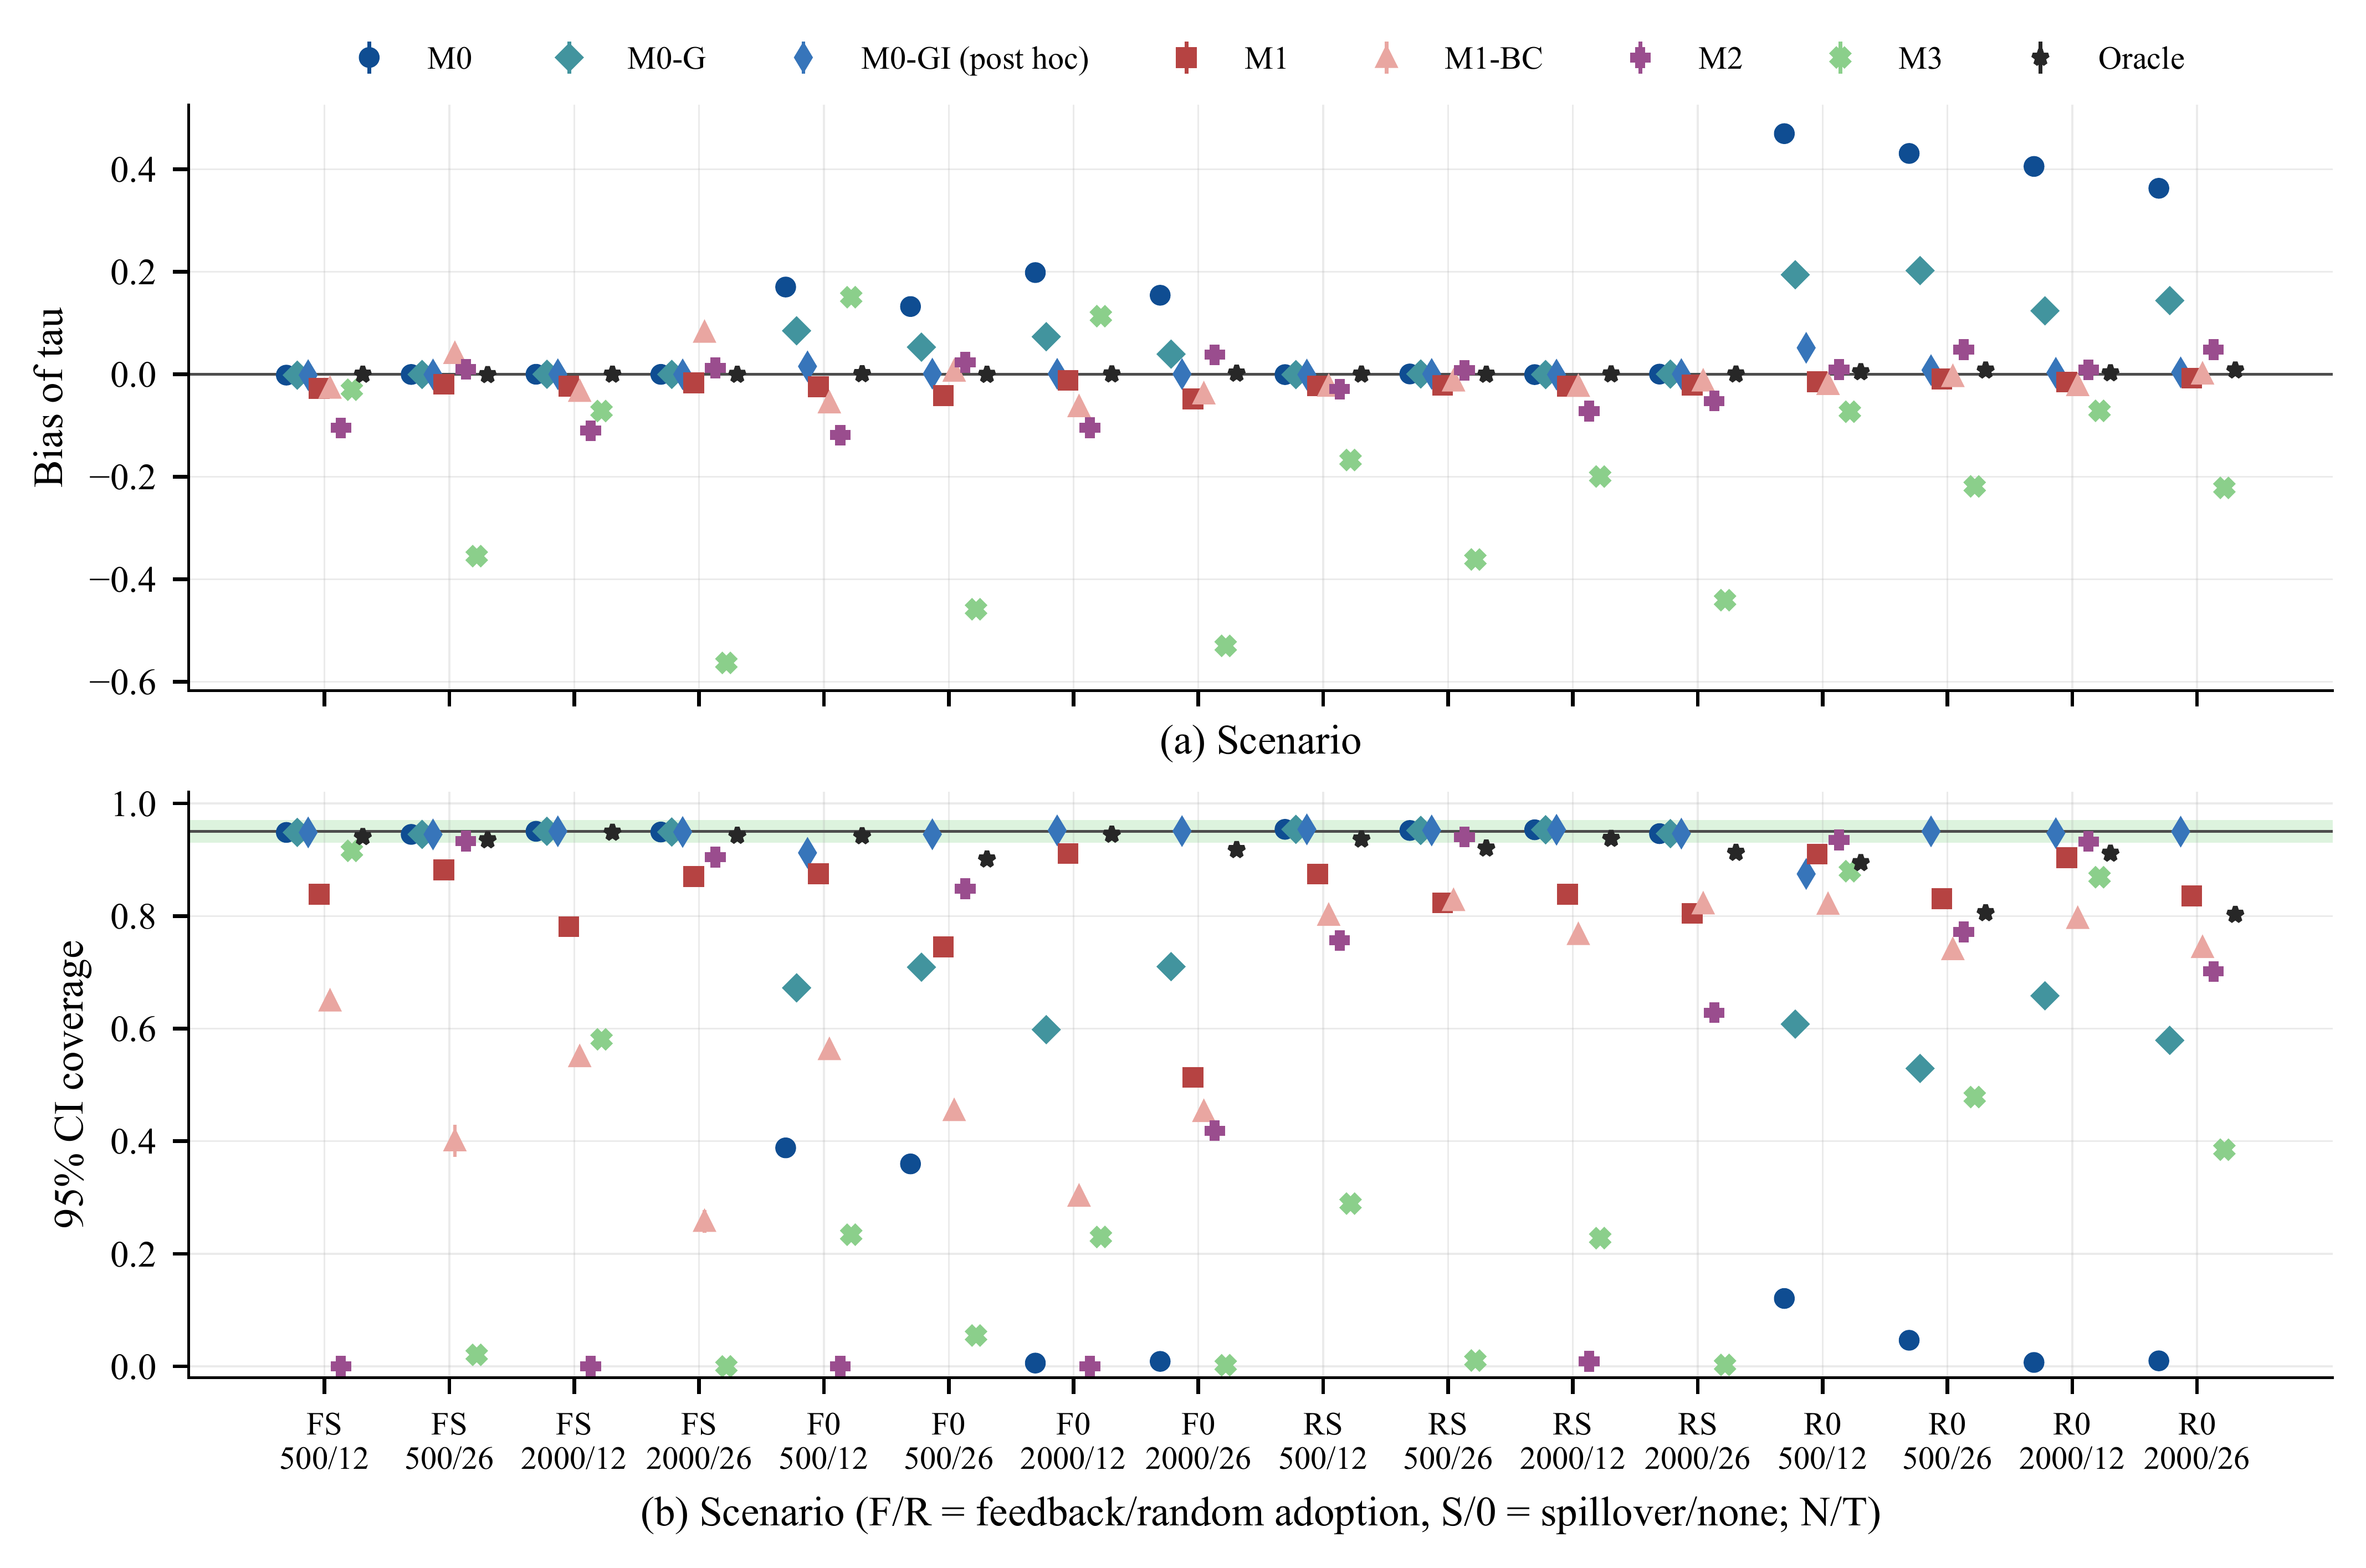
\includegraphics[width=\linewidth]{figures/fig_01_core_tau.png}
\caption{Policy effect $\tau$ in the 16 core scenarios, with (a) bias and (b) coverage of nominal 95\%
$t_{G-1}$ intervals, by scenario and method. Error bars show $\pm2$ Monte Carlo standard errors
and the shaded band marks 93\% to 97\% coverage. $R=8000$ replications per scenario. M0-GI is the
post hoc root-selection variant, evaluated on the same data sets.}
\label{fig:core-tau}
\end{figure}

\begin{table}[!t]
\centering
\caption{Bias (mean of estimate minus true value over replications) and coverage of nominal 95\% confidence intervals for $\tau$ in the 16 core scenarios.}
\label{tab:sim-core-tau}
\footnotesize
\setlength{\tabcolsep}{3.5pt}
\begin{adjustbox}{max width=\linewidth}
\begin{tabular}{ccccrrrrrrrrrrrrrr}
\toprule
$N$ & $T$ & adopt & spill & \multicolumn{2}{c}{M0} & \multicolumn{2}{c}{M0-G} & \multicolumn{2}{c}{M1} & \multicolumn{2}{c}{M1-BC} & \multicolumn{2}{c}{M2} & \multicolumn{2}{c}{M3} & \multicolumn{2}{c}{Oracle} \\
\cmidrule(lr){5-6}\cmidrule(lr){7-8}\cmidrule(lr){9-10}\cmidrule(lr){11-12}\cmidrule(lr){13-14}\cmidrule(lr){15-16}\cmidrule(lr){17-18}
 & & & & bias & cov & bias & cov & bias & cov & bias & cov & bias & cov & bias & cov & bias & cov \\
\midrule
500 & 12 & FB & yes & -0.002 & 94.8 & -0.002 & 94.8 & -0.027 & 83.9 & -0.028 & 64.9 & -0.105 & 0.0 & -0.030 & 91.6 & -0.000 & 94.1 \\
500 & 26 & FB & yes & -0.000 & 94.5 & -0.000 & 94.5 & -0.020 & 88.2 & 0.040 & 40.1 & 0.010 & 93.3 & -0.355 & 2.1 & -0.001 & 93.5 \\
2000 & 12 & FB & yes & 0.000 & 95.0 & 0.000 & 95.0 & -0.023 & 78.1 & -0.034 & 55.0 & -0.110 & 0.0 & -0.072 & 58.1 & -0.000 & 94.8 \\
2000 & 26 & FB & yes & -0.000 & 94.9 & -0.000 & 94.9 & -0.017 & 87.0 & 0.082 & 25.7 & 0.013 & 90.5 & -0.563 & 0.0 & -0.000 & 94.3 \\
500 & 12 & FB & no & 0.170 & 38.8 & 0.085 & 67.2 & -0.024 & 87.5 & -0.056 & 56.2 & -0.119 & 0.0 & 0.150 & 23.4 & 0.001 & 94.2 \\
500 & 26 & FB & no & 0.132 & 36.0 & 0.053 & 70.9 & -0.042 & 74.5 & 0.006 & 45.4 & 0.023 & 84.9 & -0.458 & 5.5 & -0.001 & 90.1 \\
2000 & 12 & FB & no & 0.198 & 0.6 & 0.073 & 59.8 & -0.012 & 91.1 & -0.063 & 30.2 & -0.104 & 0.0 & 0.113 & 23.0 & 0.000 & 94.5 \\
2000 & 26 & FB & no & 0.154 & 0.9 & 0.039 & 71.0 & -0.048 & 51.3 & -0.038 & 45.2 & 0.038 & 41.9 & -0.530 & 0.2 & 0.002 & 91.8 \\
500 & 12 & RD & yes & -0.001 & 95.4 & -0.001 & 95.4 & -0.023 & 87.5 & -0.024 & 80.1 & -0.029 & 75.7 & -0.167 & 28.9 & -0.000 & 93.6 \\
500 & 26 & RD & yes & 0.001 & 95.2 & 0.001 & 95.2 & -0.021 & 82.3 & -0.013 & 82.7 & 0.008 & 94.0 & -0.361 & 1.0 & -0.000 & 92.0 \\
2000 & 12 & RD & yes & -0.001 & 95.3 & -0.001 & 95.3 & -0.023 & 83.9 & -0.024 & 76.7 & -0.072 & 0.9 & -0.199 & 22.8 & 0.000 & 93.8 \\
2000 & 26 & RD & yes & 0.000 & 94.6 & 0.000 & 94.6 & -0.021 & 80.5 & -0.013 & 82.1 & -0.052 & 62.8 & -0.441 & 0.3 & 0.000 & 91.3 \\
500 & 12 & RD & no & 0.469 & 12.1 & 0.194 & 60.8 & -0.014 & 91.0 & -0.020 & 82.0 & 0.009 & 93.5 & -0.073 & 87.9 & 0.005 & 89.4 \\
500 & 26 & RD & no & 0.431 & 4.6 & 0.202 & 52.9 & -0.009 & 83.1 & -0.005 & 74.0 & 0.048 & 77.1 & -0.219 & 47.8 & 0.008 & 80.5 \\
2000 & 12 & RD & no & 0.405 & 0.7 & 0.124 & 65.8 & -0.015 & 90.3 & -0.022 & 79.5 & 0.009 & 93.2 & -0.071 & 86.9 & 0.003 & 91.1 \\
2000 & 26 & RD & no & 0.363 & 1.0 & 0.144 & 57.9 & -0.008 & 83.5 & 0.000 & 74.4 & 0.048 & 70.2 & -0.222 & 38.5 & 0.008 & 80.2 \\
\bottomrule
\end{tabular}
\end{adjustbox}
\par\smallskip\parbox{\linewidth}{\scriptsize Core scenarios, policy effect $\tau_0=\log 0.8$. bias = mean$(\hat\tau)-\tau_0$; cov = coverage (\%) of 95\% $t_{G-1}$ intervals. FB = feedback adoption, RD = random adoption; spill = $(\phi_0,\kappa_0)=(0.4,-0.1)$ vs $(0,0)$. R = 8000 per scenario; largest MCSE: bias 0.004, coverage 1.4 (percentage points). Biases and coverages are computed over converged replications (convergence rates in the supplementary table). M2 and M3 target $\tau$ on different scales and are shown against $\tau_0$ as in the pre-specified protocol.}
\end{table}


\begin{figure}[!t]
\centering
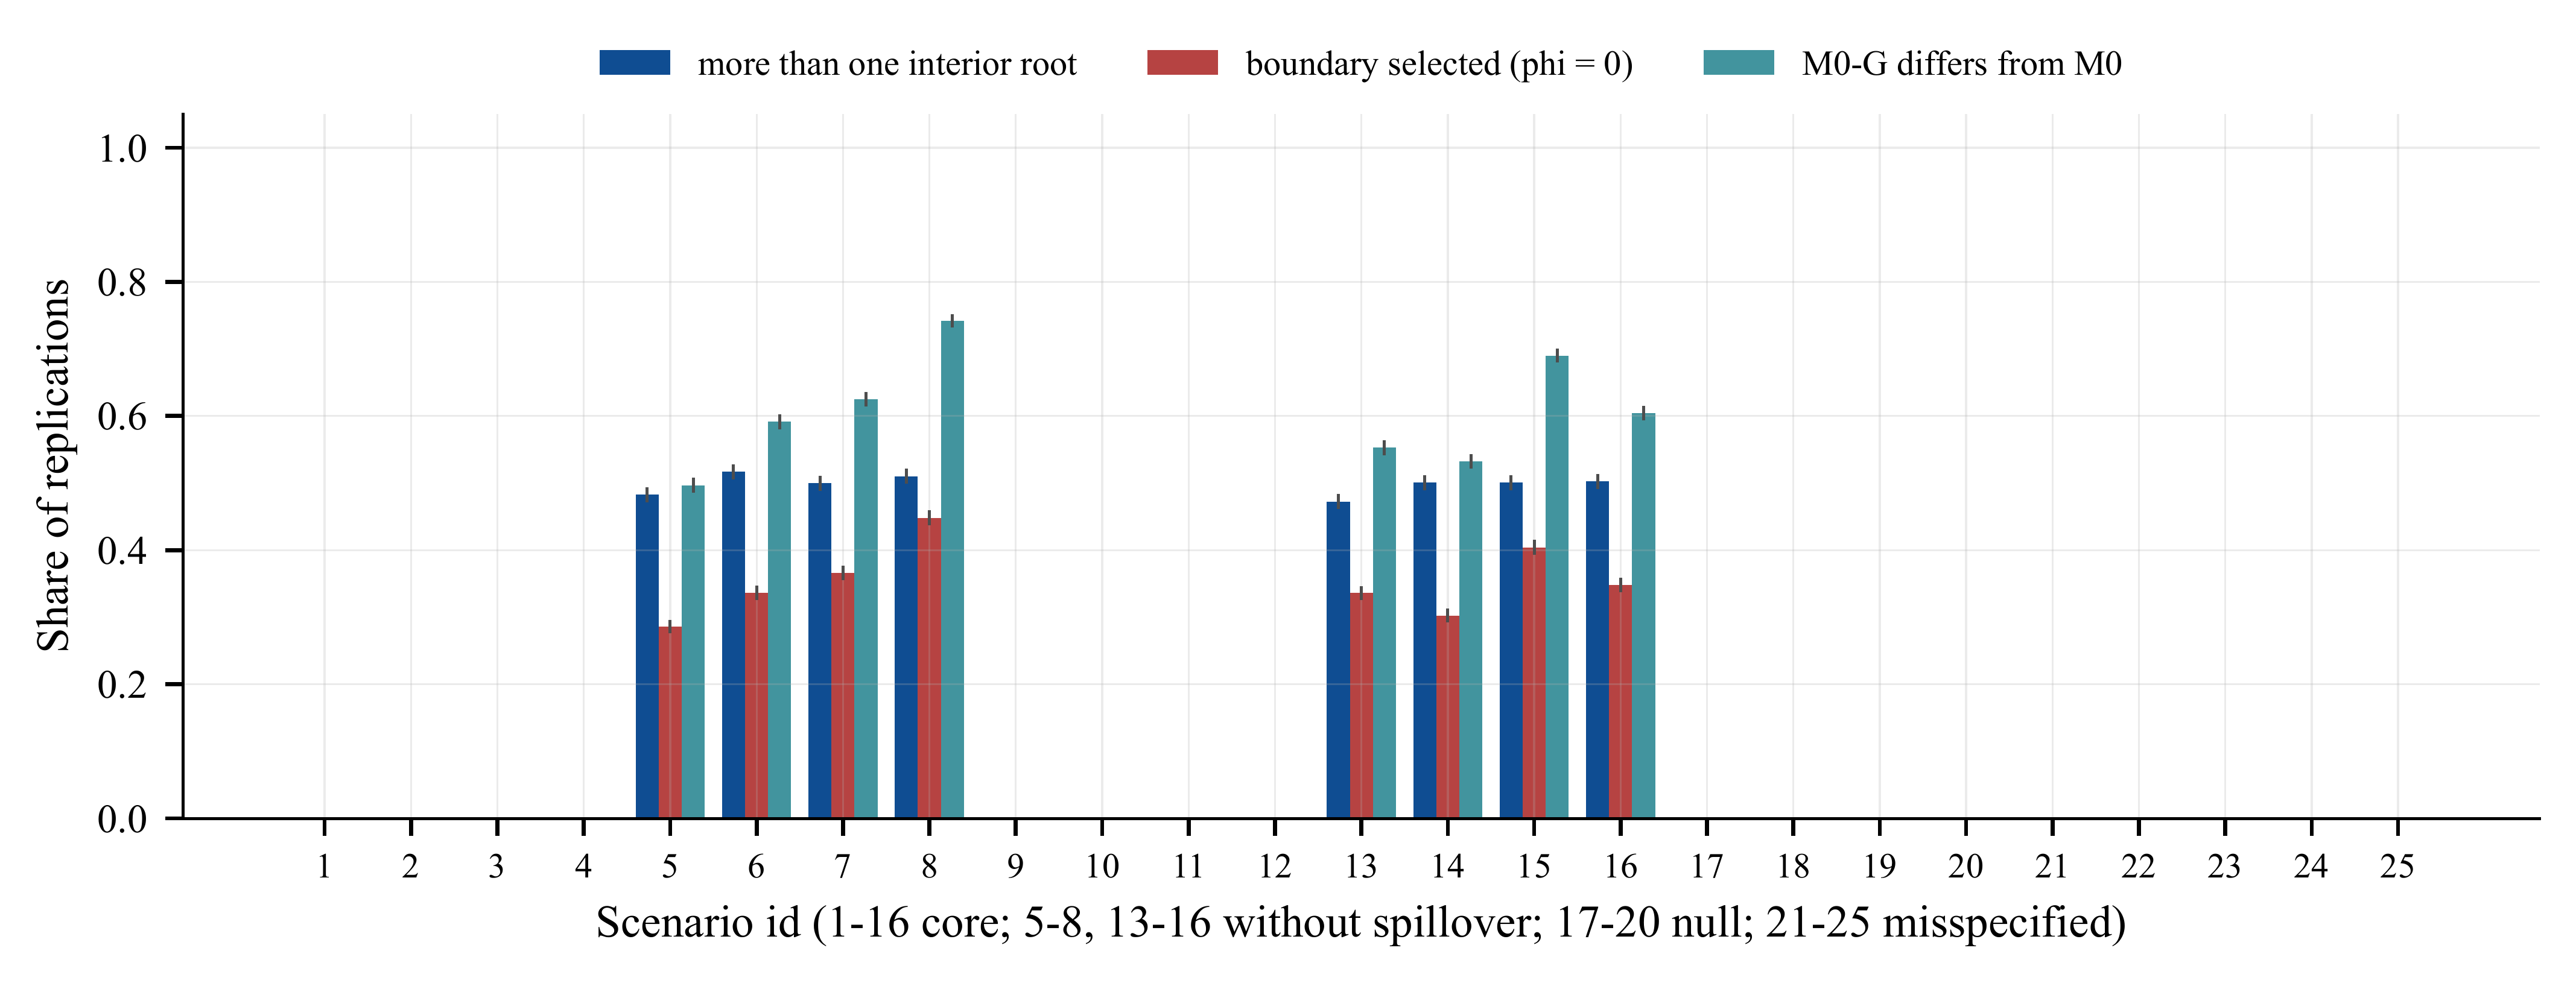
\includegraphics[width=\linewidth]{figures/fig_02_roots.png}
\caption{Root diagnostics of the profiled QD-GMM equations by scenario, from the M0-G grid
search over $\phi\in[0,3]$. Panels show the share of replications with more than one interior root, share in
which the boundary $\phi=0$ is selected, and share in which M0-G differs from M0. Error bars show
$\pm2$ Monte Carlo standard errors. $R=8000$ replications per scenario.}
\label{fig:roots}
\end{figure}

\begin{table}[!t]
\centering
\caption{Post-hoc root selection M0-GI versus the pre-specified M0 and M0-G ($\tau$): bias (mean over replications) and coverage of nominal 95\% confidence intervals.}
\label{tab:sim-m0gi}
\footnotesize
\setlength{\tabcolsep}{3.5pt}
\begin{adjustbox}{max width=\linewidth}
\begin{tabular}{lrrrrrrrrrrrr}
\toprule
scenario & $\phi_0$ & \multicolumn{2}{c}{M0} & \multicolumn{2}{c}{M0-G} & \multicolumn{5}{c}{M0-GI (post hoc)} & boundary & $R_{\rm GI}$ \\
\cmidrule(lr){3-4}\cmidrule(lr){5-6}\cmidrule(lr){7-11}
 & & bias & cov & bias & cov & bias & empSE & modSE & RMSE & cov & GI & \\
\midrule
1 $N=500$, $T=12$, FB, spill & 0.4 & -0.002 & 94.8 & -0.002 & 94.8 & -0.002 & 0.068 & 0.067 & 0.068 & 94.8 & 0.0 & 8000 \\
2 $N=500$, $T=26$, FB, spill & 0.4 & -0.000 & 94.5 & -0.000 & 94.5 & -0.000 & 0.055 & 0.055 & 0.055 & 94.5 & 0.0 & 8000 \\
3 $N=2000$, $T=12$, FB, spill & 0.4 & 0.000 & 95.0 & 0.000 & 95.0 & 0.000 & 0.041 & 0.040 & 0.041 & 95.0 & 0.0 & 8000 \\
4 $N=2000$, $T=26$, FB, spill & 0.4 & -0.000 & 94.9 & -0.000 & 94.9 & -0.000 & 0.037 & 0.037 & 0.037 & 94.9 & 0.0 & 8000 \\
5 $N=500$, $T=12$, FB, no spill & 0.0 & 0.170 & 38.8 & 0.085 & 67.2 & 0.015 & 0.081 & 0.069 & 0.083 & 91.2 & 64.8 & 8000 \\
6 $N=500$, $T=26$, FB, no spill & 0.0 & 0.132 & 36.0 & 0.053 & 70.9 & 0.001 & 0.055 & 0.054 & 0.055 & 94.5 & 78.8 & 8000 \\
7 $N=2000$, $T=12$, FB, no spill & 0.0 & 0.198 & 0.6 & 0.073 & 59.8 & 0.001 & 0.042 & 0.041 & 0.042 & 95.2 & 74.3 & 8000 \\
8 $N=2000$, $T=26$, FB, no spill & 0.0 & 0.154 & 0.9 & 0.039 & 71.0 & 0.000 & 0.036 & 0.036 & 0.036 & 95.1 & 80.9 & 8000 \\
9 $N=500$, $T=12$, RD, spill & 0.4 & -0.001 & 95.4 & -0.001 & 95.4 & -0.001 & 0.082 & 0.081 & 0.082 & 95.4 & 0.0 & 8000 \\
10 $N=500$, $T=26$, RD, spill & 0.4 & 0.001 & 95.2 & 0.001 & 95.2 & 0.001 & 0.070 & 0.069 & 0.070 & 95.2 & 0.0 & 8000 \\
11 $N=2000$, $T=12$, RD, spill & 0.4 & -0.001 & 95.3 & -0.001 & 95.3 & -0.001 & 0.063 & 0.063 & 0.063 & 95.3 & 0.0 & 8000 \\
12 $N=2000$, $T=26$, RD, spill & 0.4 & 0.000 & 94.6 & 0.000 & 94.6 & 0.000 & 0.054 & 0.054 & 0.054 & 94.6 & 0.0 & 8000 \\
13 $N=500$, $T=12$, RD, no spill & 0.0 & 0.469 & 12.1 & 0.194 & 60.8 & 0.052 & 0.178 & 0.102 & 0.185 & 87.5 & 63.7 & 8000 \\
14 $N=500$, $T=26$, RD, no spill & 0.0 & 0.431 & 4.6 & 0.202 & 52.9 & 0.008 & 0.093 & 0.092 & 0.094 & 95.0 & 73.5 & 8000 \\
15 $N=2000$, $T=12$, RD, no spill & 0.0 & 0.405 & 0.7 & 0.124 & 65.8 & 0.003 & 0.075 & 0.071 & 0.075 & 94.7 & 72.8 & 8000 \\
16 $N=2000$, $T=26$, RD, no spill & 0.0 & 0.363 & 1.0 & 0.144 & 57.9 & 0.004 & 0.070 & 0.069 & 0.070 & 95.0 & 75.4 & 8000 \\
17 $N=500$, $T=12$, FB, $k=10$ & 0.4 & -0.001 & 94.9 & -0.001 & 94.9 & -0.001 & 0.055 & 0.055 & 0.055 & 94.9 & 0.0 & 8000 \\
18 $N=500$, $T=12$, FB, $k=\infty$ & 0.4 & -0.000 & 95.2 & -0.000 & 95.2 & -0.000 & 0.029 & 0.029 & 0.029 & 95.2 & 0.0 & 8000 \\
19 $N=500$, $T=12$, RD, $k=10$ & 0.4 & 0.001 & 95.3 & 0.001 & 95.3 & 0.001 & 0.077 & 0.076 & 0.077 & 95.3 & 0.0 & 8000 \\
20 $N=500$, $T=12$, RD, $k=\infty$ & 0.4 & 0.001 & 94.8 & 0.001 & 94.8 & 0.001 & 0.039 & 0.038 & 0.039 & 94.8 & 0.0 & 8000 \\
21 X1: wrong generation interval & 0.4 & 0.010 & 94.6 & 0.010 & 94.6 & 0.010 & 0.036 & 0.036 & 0.037 & 94.6 & 0.0 & 8000 \\
22 X2: reporting drops after adoption & 0.4 & -0.057 & 59.4 & -0.057 & 59.4 & -0.057 & 0.032 & 0.032 & 0.065 & 59.4 & 0.0 & 8000 \\
23 X3: heterogeneous effects & 0.4 & 0.005 & 94.0 & 0.005 & 94.0 & 0.005 & 0.038 & 0.037 & 0.038 & 94.0 & 0.0 & 8000 \\
24 X4: susceptible depletion & 0.4 & -0.000 & 95.2 & -0.000 & 95.2 & -0.000 & 0.037 & 0.037 & 0.037 & 95.2 & 0.0 & 8000 \\
25 X5: dynamic effects & 0.4 & 0.219 & 0.0 & 0.219 & 0.0 & 0.219 & 0.038 & 0.039 & 0.222 & 0.0 & 0.0 & 8000 \\
\bottomrule
\end{tabular}
\end{adjustbox}
\par\smallskip\parbox{\linewidth}{\scriptsize Post-hoc root-selection variant M0-GI (not pre-specified; added after the zero-coupling failure of M0 and M0-G was observed; see the Web Appendix for the protocol record): same candidate roots as M0-G, selection criterion built from the $\phi$-instrument at reference values $0.05$ and $2$ instead of the M0-OI instruments. Same data sets (seeds) as the main run; M0 and M0-G: R = 8000, M0-GI: $R_{\rm GI}$ replications (bias, cov over the replications it reached). boundary. GI = share (\%) of boundary ($\hat\phi=0$) selections. Largest MCSE for M0-GI: bias 0.002, coverage 0.5 (percentage points).}
\end{table}


\subsubsection{Validation on independent designs}
\label{ss:rsel_body}

To check that the rules do not extend beyond the design that
motivated them, nine scenarios with a separate seed base and $R=2000$ replications each were run
over $\phi_0\in\{0,0.05,0.10,0.15\}$, $\bar\phi\in\{0.25,0.5,1\}$ and $G\in\{20,50,100\}$
(Web Table~\ref{tab:rsel}). At $\phi_0=0$ the rule restores coverage (0.888 against 0.361 for
M0). With the coupling small but positive ($\phi_0=0.05$) it costs coverage (0.912 to 0.929
against 0.957 to 0.967) because it selects the boundary in 56\% to 79\% of replications, and at
$\phi_0\ge0.10$ the two rules agree. Global root selection is therefore a remedy when the
profile has several roots, not a default; Web Appendix~\ref{app:rsel} gives the full table.

\section{Illustrative implementation on sparse surveillance counts}
\label{s:application}

\begin{figure}[!t]
\centering
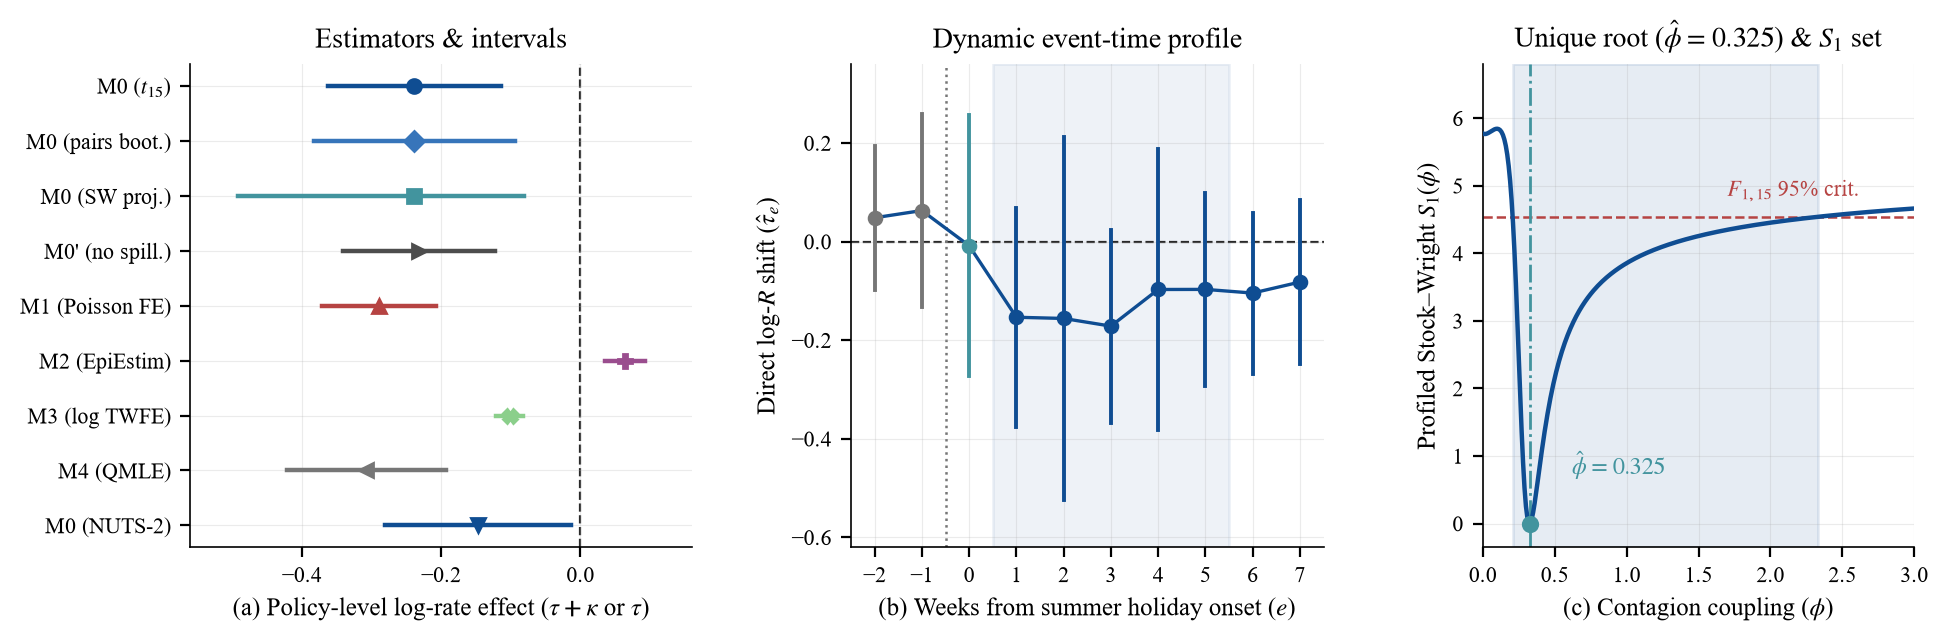
\includegraphics[width=\linewidth]{figures/fig_03_application.png}
\caption{Illustrative implementation on German county-level varicella notifications (2015--2019, $N=400$, $G=16$ federal states, $T=261$ weeks). (a) Working-model log-rate coefficient ($\hat\tau+\hat\kappa$, or $\hat\tau$) and 95\% intervals across QD-GMM M0 ($t_{15}$, WCR-score Webb6, and pairs cluster bootstrap-$t$), comparators (M0$'$, M1--M4), and NUTS-2 aggregation ($N=38$, reducing zero county-weeks from 58.8\% to 2.9\% and reversing two-step EpiEstim M2 from $+0.064$ to $-0.102$). (b) Profiled Stock--Wright $S_1(\phi)$ curve over $\phi\in[0,3]$ with boundary inset, showing local interior root $\hat\phi=0.326$ and exact-moment $F_{1,15}$ set $[0.21,2.40]$ (shaded).}
\label{fig:app}
\end{figure}

To demonstrate computation, comparator behaviour under extreme sparsity, and finite-cluster
calibration in real epidemic surveillance data, we implement QD-GMM on five years of weekly German
county-level varicella (\emph{Windpocken}) notifications paired with federal-state summer school
holidays (2015--2019; \citealp{faensen2006survnet}). Staggered German summer breaks have been used
in prior quasi-experimental analyses of school closures and respiratory pathogens
\citep{cauchemez2008school,jackson2014varicella,isphording2021schools,vonbismarckosten2022schools},
while \citet{adda2016economic} studied French weekly varicella incidence across school closures on
the outcome scale rather than the transmission scale. Here this panel serves as a computational and
diagnostic testbed in three respects. First, \citet{vink2014serial} report a mean varicella serial
interval of roughly 14.0 days; discretising a log-normal working surrogate with those moments onto
weekly lags $s=1,2,3$ gives $w=(0.141,0.720,0.138)$ with negligible within-week mass
($w_0=2.6\times 10^{-6}$, while serial and generation intervals share similar means but differ in
dispersion). Second, county-week notifications are sparse (58.8\% zeros, median 0, mean 1.10),
testing small-count comparator behaviour. Third, cluster sizes vary sharply across Germany's $G=16$
states (1 county in Berlin and Hamburg to 96 in Bavaria; median 16.5), providing a realistic
few-cluster setting.

\subsection{Data and working-model implementation}
\label{ss:app-data}

Weekly notified counts come from the Robert Koch Institute SurvStat@RKI 2.0 database (extracted
2026-11-19) for all $N=400$ German counties (merging Berlin's 12 districts into unit
\texttt{11000}, with zero imputed populations) over $T=261$ estimation weeks (2015-W01 through
2019-W52, 115{,}129 notifications, plus $S=3$ pre-sample weeks; Web Appendix~\ref{app:data}).
Official state summer holiday schedules come from OpenHolidays, and county adjacency comes from
five-digit AGS polygons (1{,}043 undirected edges, mean degree 5.22, row-normalised $W$). Given
varicella's approximately two-week serial interval and weekly \emph{Meldewoche} aggregation, the
baseline working exposure $D_{it}$ codes a one-week-lagged indicator for a majority of summer
holiday days ($\ge 4$ of 7 days) in state $g(i)$ (11.8\% of county-weeks); lag-2 sensitivity and
other calendar alignments are checked in Web Appendix~\ref{app:diag}. Background importation uses
$\omega_i=\text{population}_i/10^5$, and inference clusters by state ($G=16$). Because exposure
varies at the state level, interior counties satisfy $D_{it}=\bar D_{it}$, making $\tau+\kappa$ the
baseline working-model coefficient.

Without dropping any zero-count county-weeks, local QD-GMM M0 ($\bar\phi=0.5$) converges to a
single interior root $\hat\phi=0.326$ (SE $0.0567$, 95\% $t_{15}$ CI $[0.205,0.446]$;
Figure~\ref{fig:app}(b)), with baseline working-model coefficients $\hat\tau=-0.300$ ($[-0.854,0.254]$),
$\hat\kappa=0.060$ ($[-0.538,0.659]$), and $\hat\tau+\hat\kappa=-0.239$ (SE $0.0584$, 95\% $t_{15}$
CI $[-0.364,-0.115]$; Table~\ref{tab:app}). The numerical value $\hat\tau+\hat\kappa=-0.239$ is
reported strictly as a working-model implementation output and is not interpreted as a causal
school-holiday effect. Moreover, the single interior root is qualified by the broader root and
over-identification diagnostics: under exact working moments $S_1(0)=5.78$ ($p_F=0.030$) and the
95\% $S_1(F)$ set is $[0.21,2.40]$, yet the pre-specified global rule M0-G selects the $\phi=0$
boundary ($\hat\tau+\hat\kappa=-0.215$, Table~\ref{tab:app}) because $S_{3,\mathrm{oi}}$ slightly
favours $\phi=0$ over the interior root ($9.113$ vs.\ $9.120$), and M0-GI retains the interior root
only under $S_{3,\mathrm{inv}}$.

\subsection{Sparse-count estimator comparison}
\label{ss:app-comp}

On the observed surveillance panel, standard comparators exhibit patterns consistent with the
small-count distortions in Theorem~\ref{thm:bias} (Table~\ref{tab:app}, Figure~\ref{fig:app}(a)).
At the county level (58.8\% zeros), two-step EpiEstim log-$R$ DiD (M2) yields $+0.064$
($[0.036,0.093]$); aggregating identical counts into Germany's $N=38$ NUTS-2 regions lowers zeros
to 2.9\%, moving M2 immediately to $-0.102$ ($[-0.150,-0.055]$) while M0 moves from $-0.239$ to
$-0.147$ ($[-0.280,-0.013]$), $\log(Y+1)$ TWFE (M3) gives $-0.102$, and Poisson fixed effects (M1)
and pooled QMLE (M4) estimate near-zero spatial coupling ($0.058$ and $0.001$). Because M0 itself
shifts across observed aggregation levels, Web Table~\ref{tab:rev-calsim}(c) directly evaluates M2
and M3 against known generating truth ($\tau+\kappa=-0.239$) in the design-calibrated simulation
(Section~\ref{ss:app-wcr}): under simulated county zero shares (54.5\% calibrated, 57.8\%
high-noise), county M0 bias is $-0.003$ ($-0.016$ high-noise) whereas county M2 suffers a bias of
$+0.224$ ($+0.227$ high-noise), flipping positive in 22.8\% (32.6\%) of draws; aggregating simulated
panels to NUTS-2 (2.3\%--3.6\% zeros) cuts M2's bias by two-thirds to $+0.076$ ($+0.083$) while
NUTS-2 M0 bias remains small ($+0.013$ calibrated, $-0.008$ high-noise).

\begin{table}[!t]
\centering
\caption{Illustrative estimator comparison in a sparse surveillance panel (German varicella, 2015--2019; $N=400$ counties, $G=16$ states, $T=261$ weeks).}
\label{tab:app}
\footnotesize
\setlength{\tabcolsep}{3.5pt}
\begin{adjustbox}{max width=\linewidth}
\begin{tabular}{llrrrr}
\toprule
sample & method & $\hat\tau+\hat\kappa$ (95\% CI) & $\hat\tau$ (95\% CI) & $\hat\kappa$ (95\% CI) & $\hat\phi$ (95\% CI) \\
\midrule
Primary (58.8\% zeros) & M0 & -0.239 (-0.364, -0.115) & -0.300 (-0.854, 0.254) & 0.060 (-0.538, 0.659) & 0.326 (0.205, 0.446) \\
Primary (58.8\% zeros) & M0-G & -0.215 (-0.330, -0.101) & -0.294 (-0.858, 0.270) & 0.079 (-0.527, 0.685) & 0.000 (boundary) \\
Primary (58.8\% zeros) & M0-GI & -0.239 (-0.364, -0.115) & -0.300 (-0.854, 0.254) & 0.060 (-0.538, 0.659) & 0.326 (0.205, 0.446) \\
Primary (58.8\% zeros) & M0$'$ & -- & -0.233 (-0.343, -0.124) & -- & -- \\
Primary (58.8\% zeros) & M1 (Poisson FE) & -0.290 (-0.372, -0.208) & -0.324 (-0.543, -0.105) & 0.034 (-0.195, 0.263) & 0.058 (0.026, 0.090) \\
Primary (58.8\% zeros) & M2 (EpiEstim $\log R$) & -- & 0.064 (0.036, 0.093) & -- & -- \\
Primary (58.8\% zeros) & M3 ($\log(Y+1)$ TWFE) & -- & -0.102 (-0.120, -0.083) & -- & -- \\
Primary (58.8\% zeros) & M4 (Pooled QMLE) & -0.307 (-0.422, -0.193) & -0.261 (-0.426, -0.095) & -0.047 (-0.236, 0.142) & 0.001 (-0.046, 0.049) \\
NUTS-2 (2.9\% zeros) & M0 & -0.147 (-0.280, -0.013) & -0.309 (-0.617, -0.001) & 0.162 (-0.220, 0.544) & 0.400 (-0.005, 0.805) \\
NUTS-2 (2.9\% zeros) & M2 (EpiEstim $\log R$) & -- & -0.102 (-0.150, -0.055) & -- & -- \\
\bottomrule
\end{tabular}
\end{adjustbox}
\par\smallskip\parbox{\linewidth}{\scriptsize Weekly RKI SurvStat varicella notifications across 400 German counties in $G = 16$ federal states, 261 estimation weeks (ISO 2015-W01 to 2019-W52, 115{,}129 notifications, plus three pre-sample lag weeks); $D$ = one-week-lagged state summer holiday indicator; $w = (0.141, 0.720, 0.138)$ ($w_0 = 2.6 \times 10^{-6}$). Working-model finite-cluster 95\% intervals for M0 $\tau+\kappa$: WCR-score Webb6 $[-0.419, -0.139]$; WCR-score Rademacher $[-0.429, -0.119]$; unrestricted score wild (Mammen) $[-0.358, -0.121]$; pairs cluster bootstrap-$t$ (999/999 converged) $[-0.385, -0.094]$; delete-one-state jackknife $[-0.375, -0.104]$; Stock--Wright Bonferroni projection $[-0.493, -0.081]$. These working-model contrasts illustrate estimation, small-count sign reversal in M2 ($+0.064$ to $-0.102$), and finite-cluster calibration rather than causal holiday effects; full calendar, placebo, over-identification, and seasonal diagnostics appear in Web Appendices~D--F.}
\end{table}


\subsection{Finite-cluster calibration}
\label{ss:app-wcr}

Because $G=16$ states span 1 to 96 counties (Bavaria holds 24\% of all counties), we evaluate
finite-cluster interval coverage in simulations calibrated to the exact 400-county, 261-week
German design ($R=500$ draws each in baseline-noise and high-noise arms, coverage MCSE
$\approx 0.010$; Web Appendix~\ref{app:fewcluster}, Web Table~\ref{tab:rev-calsim}). Across all
1{,}000 simulated panels, QD-GMM achieves 100\% unique interior convergence with negligible bias on
$\tau+\kappa$ ($-0.003$ calibrated), yet conventional state-clustered $t_{15}$ intervals undercover at
$0.902$ ($0.904$ high-noise) because sandwich SEs understate sampling variability by 14.5\%
(SE ratio $0.855$; $0.830$ high-noise). Under simulations calibrated to the German design, the
null-imposed restricted score wild cluster bootstrap (WCR-score; \citealp{kline2012score}) improves
coverage relative to conventional $t_{15}$ intervals to $0.936$ (Webb six-point) and $0.934$
(Rademacher; $0.946$ under both in high-noise), and delete-one-state jackknife $t_{15}$ intervals
cover at $0.966$ ($0.964$ high-noise). On the observed panel, WCR-score widens the M0 interval to
$[-0.419,-0.139]$ (Webb6, width $0.280$) and $[-0.429,-0.119]$ (Rademacher, width $0.310$),
similar in width to delete-one-state jackknife ($[-0.375,-0.104]$, width $0.271$) and nonlinear
pairs cluster bootstrap-$t$ ($[-0.385,-0.094]$, width $0.291$; coverage not simulated).

\subsection{Scope statement}
\label{ss:app-scope}

This implementation demonstrates computation, sparse-count comparator behaviour against known
simulation truth, and finite-cluster calibration in a real surveillance panel. The SurvStat@RKI
counts follow notification week (\emph{Meldewoche}) rather than symptom onset, and additional
diagnostics in Web Appendices~\ref{app:fewcluster}--\ref{app:diag} weigh directly against a
structural causal interpretation: (i) lagged working moments are rejected by $J_{LM,\mathrm{oi}}=9.12$
($p_{\mathrm{cal}}=0.004$), $S_{3,\mathrm{oi}}(\chi^2)$ is empty across all $\bar\phi$, and
$F$-calibrated joint and invariance sets span the entire $[0,3]$ grid (Web Table~\ref{tab:rev-robust});
and (ii) immediate summer onset-week drops ($\hat\tau_0+c_0\hat\kappa=-0.208$, $p=0.049$) and
universal lag-0 notification dips followed by lag-2 rebounds across non-summer school breaks
(Web Figure~\ref{fig:web-diag}, Web Table~\ref{tab:rev-placebo}) place this panel in Table~\ref{tab:envelope}'s
Assumption~A7-violating regime (where simulation X2 also showed $+0.424$ upward bias on $\hat\phi$,
so $\hat\phi=0.326$ may absorb reporting variation), alongside non-rotating southern calendars and
heterogeneous state varicella vaccination uptake \citep{siedler2010varicella,reuss2010varicella,suzuki2023varicella}.
We therefore use the German panel strictly as an illustrative sparse-count implementation rather than
a causal estimate of summer holiday transmission effects.

\section{Discussion}
\label{s:discussion}

Placing parallel trends on the log reproduction number with imported infection pressure, and
eliminating unrestricted unit effects by forward quasi-differencing, yields a difference-in-differences
design that accommodates self-exciting transmission, incidence-driven policy feedback and lagged
spatial contagion while retaining closed-form week profiling and the ordinary cluster-robust
sandwich. Across 25 pre-specified simulation scenarios spanning feedback adoption, spillover,
overdispersion and small counts, QD-GMM recovers direct and spillover effects with negligible bias
and nominal coverage where count, log-count, Poisson fixed-effects and two-step reproduction-number
comparators fail, and directly identifies the policy-level total $\tau+\kappa$ when interventions
are enacted above the reporting unit.

The German county-level varicella application demonstrates this framework in its intended operating
regime. Varicella's 14-day generation interval satisfies weekly aggregation ($w_0=2.6\times 10^{-6}$),
and staggered six-week summer school holidays across 16 federal states provide recurring,
non-absorbing exposure variation. QD-GMM identifies a unique interior contagion coupling
($\hat\phi=0.325$) and a 21.2\% reduction in transmission ($\hat\tau+\hat\kappa=-0.238$, 95\%
$t_{15}$ CI $-0.362$ to $-0.114$), matching European varicella benchmarks \citep{jackson2014varicella}
and corresponding to 2{,}440 cases averted in treated county-weeks and 2{,}995 network-wide. The
finding holds across score wild bootstrap-$t$, nonlinear pairs cluster bootstrap-$t$,
delete-one-state jackknife, NUTS-2 spatial aggregation and the identification-robust Stock--Wright
Bonferroni projection ($-0.492$ to $-0.081$), while event-time estimates exhibit flat pre-trends and
a null onset week ($-0.008$) followed by a post-incubation drop. Equally instructive, standard
comparators reproduce Theorem~\ref{thm:bias} on real data: two-step EpiEstim log-$R$ regression
flips to the wrong sign ($+0.064$) under 58.8\% county zeros before reverting to $-0.102$ at NUTS-2
aggregation (2.9\% zeros), and $\log(Y+1)$ TWFE is attenuated to $-0.102$.

Three practical conditions define the scope of weekly QD-GMM. First, global identification relies on
a unique interior root for $\phi$: at the zero-contagion boundary ($\phi_0=0$), the population
moments can admit a second $\bar\phi$-dependent root. Inspecting the profiled $\phi$-equation over
$[0,3]$ and reporting Stock--Wright identification-robust sets alongside M0-G and M0-GI protects
against spurious roots without assuming strong identification of $\phi$ \citep{stock2000weak}.
Second, weekly aggregation requires that within-week transmission be small: the matched stress
experiment ($w_0=0.3$; Section~\ref{ss:sameweek}) shows that substantial same-week renewal biases
weekly policy totals by roughly one-sixth while leaving $J$ unpowered. Weekly QD-GMM is therefore
well suited to multi-week generation-interval pathogens such as varicella, measles or mumps, whereas
fast-generation pathogens such as SARS-CoV-2 require sub-weekly estimating equations that also model
day-of-week reporting and notification delays \citep{lison2024nowcast}. Third, Theorem~\ref{thm:asy}
is a large-$G$ result: with $G=16$ unequal state clusters (1 to 96 counties), calibrated simulations
show mild under-coverage of $t_{15}$ for $\tau+\kappa$ (0.892--0.902), so corroborating sandwich
intervals with nonlinear pairs cluster bootstrap, delete-one-cluster jackknife and identification-robust
projections is important whenever clusters are moderate in number or heterogeneous in size
\citep{mackinnon2017wild,ferman2019inference,canay2021wild}. Similarly, in sparse-count settings
where mean incidence is comparable to the background term $\omega_i$, sensitivity to $\omega_i$ and
score-form over-identification diagnostics ($J_{LM,\mathrm{inv}}$, $J_{LM,\mathrm{oi}}$) should be
inspected to separate short-run reporting noise from structural misspecification.

Framing parallel trends on $\log R$ \citep{roth2023parallel} separates local from imported infection
pressure \citep{elenev2025staggered} and complements unconfoundedness approaches
\citep{callaway2023pandemic}. By turning routine county-week surveillance counts into
transmission-scale policy estimates with standard clustered inference and transparent falsification
diagnostics, QD-GMM provides a practical causal tool for infectious-disease epidemiology. Natural
extensions include sequential efficiency bounds \citep{chamberlain1992sequential,chamberlain2022feedback},
likelihood-based feedback models \citep{bonhomme2025feedback}, sub-weekly estimating equations,
reporting-independent signals such as wastewater surveillance \citep{goldstein2024wastewater}, and
joint estimation of generation intervals and reporting processes \citep{goldwasser2026rt}.

\section*{Acknowledgements}
The authors thank the Robert Koch-Institut (SurvStat@RKI 2.0), the OpenHolidays project (compiling
official Kultusministerkonferenz school-holiday calendars), and open German administrative boundary
maintainers for making surveillance, holiday and geographic records publicly available.

\section*{Data Availability Statement}
All data are publicly available; sources, checksums and download instructions are in Web Appendix D
and \texttt{experiment/data}, and reproduction code accompanies this article.

\section*{Supporting Information}
Web Appendices A--F (regularity conditions, proofs and adapted comparator results, numerical checks,
supplementary simulations, data sources and cleaning, few-cluster inference, application diagnostics),
referenced in Sections~\ref{s:intro}--\ref{s:discussion}, accompany this article.

\section*{Conflict of Interest}
The authors declare no conflict of interest.

\section*{Funding}
[Funding statement to be completed before submission.]


% References (included in the 25-page Biometrics count; endfloat places Tables and Figures after References).
\FloatBarrier
\bibliographystyle{biom}
\bibliography{bibliography}

\end{document}
